% !TEX program = xelatex
% =====================================================================
%  操作系统课程设计报告 —— UNIX V6++ 离散化内存管理
%  参照学长报告(白佳煜, 2352733)结构搭建的 LaTeX 全文架构
%  编译: latexmk -xelatex main.tex   (或 xelatex 连续两次)
% =====================================================================
\documentclass[a4paper,11pt,openany,UTF8]{ctexbook}

% ---------- 页面与版式 ----------
\usepackage[a4paper,top=2.5cm,bottom=2.5cm,left=2.5cm,right=2.5cm]{geometry}
\usepackage{fancyhdr}
\usepackage{titlesec}

% ---------- 中文与字体 ----------
% ctexbook 已处理中文; xelatex 下默认使用系统字体, 可按需在下方覆盖
% \setCJKmainfont{SimSun}   % 如需指定正文字体, 取消注释

% ---------- 排版增强 ----------
\usepackage{graphicx}
\usepackage{float}
\usepackage{caption}
\usepackage{subcaption}
\usepackage{booktabs}
\usepackage{array}
\usepackage{longtable}
\usepackage{multirow}
\usepackage{enumitem}
\usepackage{tabularx}
\usepackage{amsmath,amssymb}

% ---------- 代码清单 ----------
\usepackage{listings}
\usepackage{xcolor}
\usepackage{chngcntr}

% ---------- 超链接 ----------
\usepackage[colorlinks=true,linkcolor=black,citecolor=blue,urlcolor=blue]{hyperref}

% =====================================================================
%  封面信息 (请按实际情况修改)
% =====================================================================
\newcommand{\ReportTitle}{操作系统课程设计报告}
\newcommand{\ReportSubtitle}{UNIX V6++ 离散化内存管理}
\newcommand{\StudentName}{\textbf{韦畅}}        % TODO: 姓名
\newcommand{\StudentId}{\textbf{2352628}}          % TODO: 学号
\newcommand{\Department}{计算机科学与技术学院}
\newcommand{\Major}{计算机科学与技术}
\newcommand{\Advisor}{方钰}
\newcommand{\ReportDate}{2026 年 \the\month\ 月}

% =====================================================================
%  代码清单样式 (学长报告使用 Listing X.Y 风格)
% =====================================================================
\definecolor{codegray}{rgb}{0.5,0.5,0.5}
\definecolor{codeblue}{rgb}{0.0,0.0,0.6}
\definecolor{codegreen}{rgb}{0.0,0.5,0.0}
\definecolor{codebg}{rgb}{0.97,0.97,0.97}

\lstset{
    basicstyle=\ttfamily\small,
    keywordstyle=\color{codeblue}\bfseries,
    commentstyle=\color{codegray}\itshape,
    stringstyle=\color{codegreen},
    numberstyle=\tiny\color{codegray},
    numbers=left,
    numbersep=8pt,
    frame=single,
    framesep=5pt,
    rulecolor=\color{codegray!50},
    backgroundcolor=\color{codebg},
    breaklines=true,
    breakatwhitespace=true,
    showstringspaces=false,
    tabsize=4,
    captionpos=b,
    abovecaptionskip=6pt,
    xleftmargin=12pt,
    language=C++,
}
% 代码清单按章编号, 显示为 "代码清单 3.1"
\renewcommand{\lstlistingname}{代码清单}
\AtBeginDocument{\counterwithin{lstlisting}{chapter}}

% 图表按章编号 (图 3-1 / 表 4-1), 用连字符更贴近学长风格
\renewcommand{\thefigure}{\arabic{chapter}-\arabic{figure}}
\renewcommand{\thetable}{\arabic{chapter}-\arabic{table}}

% 运行截图占位框: 正文成稿前用占位标记截图位置, 运行后替换为 \includegraphics
\newcommand{\shotbox}[1]{%
  \begin{center}%
  \fcolorbox{gray!60}{gray!10}{%
    \parbox[c][3.6cm][c]{0.82\textwidth}{\centering\itshape
      【运行截图占位】\\[2pt]\normalfont #1\\[2pt]\itshape (运行后替换为实际截图)}}%
  \end{center}}

% =====================================================================
%  页眉页脚
% =====================================================================
\pagestyle{fancy}
\fancyhf{}
\fancyhead[L]{\small 操作系统课程设计报告}
\fancyhead[R]{\small UNIX V6++ 离散化内存管理}
\fancyfoot[C]{\thepage}
\renewcommand{\headrulewidth}{0.4pt}

% 章节标题样式
\titleformat{\chapter}[block]{\huge\bfseries\centering}{第\zhnum{chapter}章}{1em}{}
\titlespacing*{\chapter}{0pt}{-20pt}{30pt}

% 消除 \cleardoublepage 产生的空白页 (封面后/参考文献后等); 让其等价于 \clearpage
\let\cleardoublepage\clearpage

% =====================================================================
%  文档开始
% =====================================================================
\begin{document}

% ---------- 封面 ----------
% =====================================================================
%  封面页 —— 参照同济大学操作系统课程设计报告格式 (单页)
% =====================================================================
\begin{titlepage}
\thispagestyle{empty}
\centering
\vspace*{1cm}

{\zihao{2}\textbf{\ReportTitle}}

\vspace{0.8cm}
{\zihao{3}\textbf{\ReportSubtitle}}

\vspace{1.8cm}

\includegraphics[width=0.25\textwidth]{figures/logo.png}

\vspace{1.8cm}

{\zihao{3}
\renewcommand{\arraystretch}{1.6}
\begin{tabular}{rl}
学\quad 院： & \Department \\
专\quad 业： & \Major \\
姓\quad 名： & \StudentName \\
学\quad 号： & \StudentId \\
指导教师：   & \Advisor \\
\end{tabular}}

\vfill
{\zihao{3}\ReportDate}
\vspace*{1cm}

\end{titlepage}


% ---------- 目录 ----------
\frontmatter
\cleardoublepage
\phantomsection
\addcontentsline{toc}{chapter}{目录}
\tableofcontents

% ---------- 正文 ----------
\mainmatter
% =====================================================================
%  第一章  绪论
% =====================================================================
\chapter{绪论}

\section{课设背景与意义}
操作系统是计算机系统中最为核心的系统软件，而内存管理又是操作系统中牵涉面最广、
与其他子系统耦合最深的模块之一。进程的创建与切换、可执行程序的加载、异常与缺页
处理、设备 I/O 缓冲，乃至系统调用时内核对用户态地址的访问，都建立在内存管理所
维护的地址映射之上。正因如此，对内存管理机制的深入理解，往往是从"会用操作系统"
迈向"理解操作系统"的关键一步。

UNIX V6 及其衍生版本长期以来都是操作系统教学的经典载体。Lions 的《UNIX 操作系统
源代码注释》以不到一万行的内核代码完整展示了一个真实操作系统的全貌，而同济大学
在 UNIX V6 基础上改造的 UNIX V6++ 进一步将其移植到 32 位保护模式，引入了基于
80386 的页式内存管理，使其更贴近现代操作系统的实现方式。本次课程设计即以 UNIX V6++
为平台，聚焦于其内存管理子系统的改造。

原 UNIX V6++ 的内存管理以\textbf{连续进程映像}为基础：一个进程的用户态图像
（代码段、数据段、栈段）在物理内存中占据一段连续区域，进程创建时需要整体复制
父进程图像，内存不足时则通过盘交换区（swap）把进程图像换出到磁盘。这种"连续
分配 + 盘交换"的模型虽然在概念上直观，却与现代操作系统普遍采用的\textbf{请求分页
+ 离散分配}模型相去甚远。本次课设的目标，正是把 UNIX V6++ 的内存管理从连续映像
模型改造为以 4KB 页框为单位的离散化管理模型，并在改造过程中不依赖盘交换区。
这一改造既是对分页机制本身的一次完整实践，也使得进程创建、程序加载等关键路径
能够采用写时复制（Copy-On-Write）、按需分配等更高效的策略，具有明显的教学与
工程价值。

\section{原系统内存管理概述}
在展开改造方案之前，有必要先回顾原 UNIX V6++ 内存管理的基本面貌，这也是本次
课设的改造对象。原系统的虚实地址空间分布如下（沿课设 PPT 的描述）：物理内存自低地址起依次划分为保留区（0\,–\,1M）、内核
（1M 起）、内核堆对象区（1.5M 起）、页表区（2M 起）和用户区（4M 起）；用户进程
的虚地址空间则包含代码段、数据段、堆栈段等区域。

\begin{figure}[H]
  \centering
  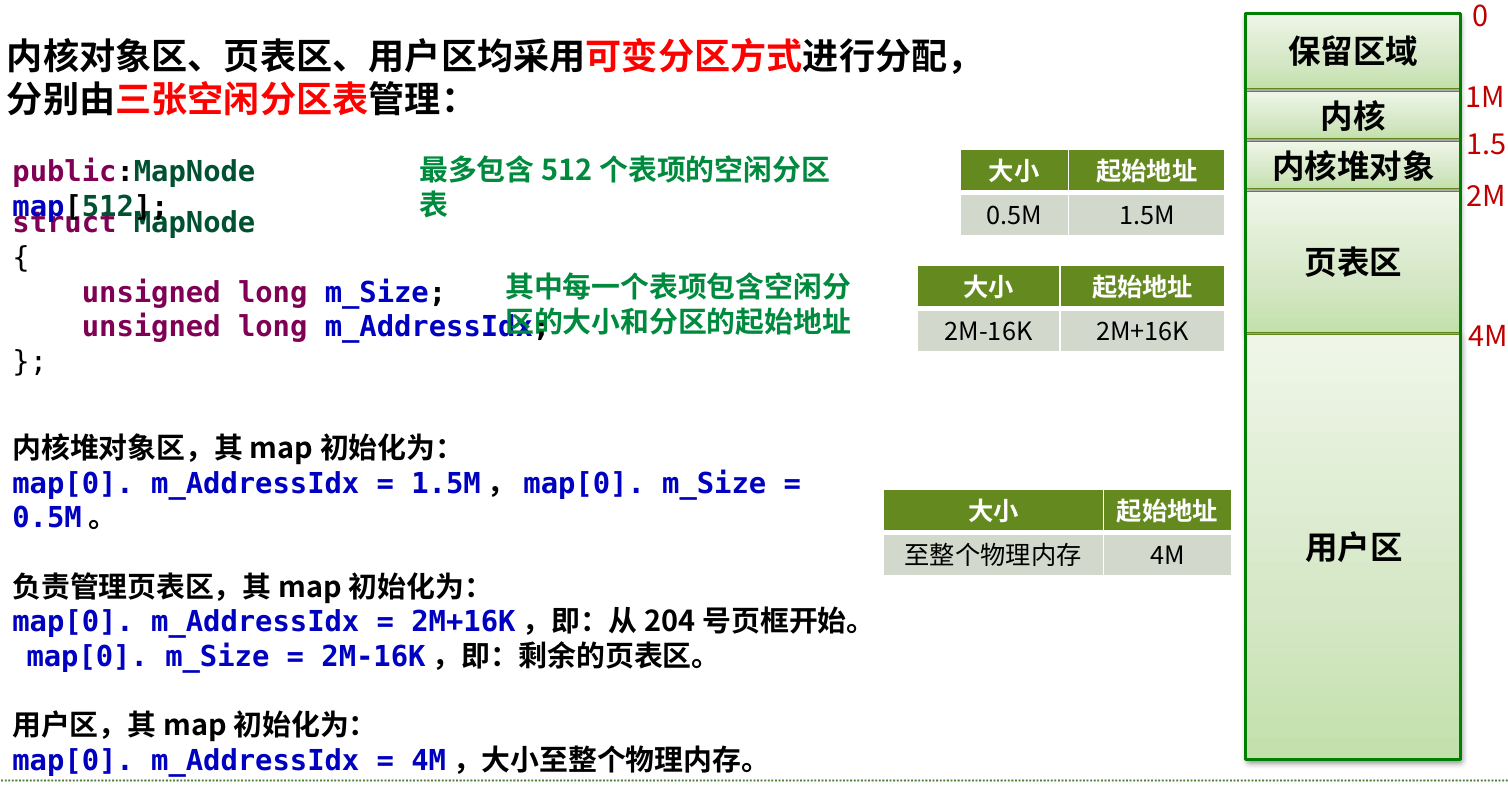
\includegraphics[width=0.85\textwidth]{figures/fig_mem_layout.png}
  \caption{UNIX V6++ 物理内存地址空间布局（图源：课程设计 PPT slide 21）}
  \label{fig:mem-layout}
\end{figure}

在\textbf{分配方式}上，原系统采用连续可变分区管理，由一张最多 512 个表项的
空闲分区表 \texttt{MapNode map[512]} 记录各空闲分区的大小与起始地址，分配算法
\texttt{Allocator::Alloc/Free}（对应 UNIX V6 中的 \texttt{malloc/mfree}）实现
首次适配与相邻分区合并。内核堆对象区、页表区、用户区分别由各自的分区表管理。

在\textbf{进程图像}上，原系统为每个进程维护一段连续的物理内存用于存放其用户态
图像，进程控制块 \texttt{Proc} 中的 \texttt{p\_addr} 字段指向该连续区域的起始
地址。其结果是：\texttt{fork} 创建子进程时需要把父进程的整段图像复制一遍；
\texttt{exec} 加载新程序时需要为其分配一段足够大的连续内存；当物理内存不足以
容纳所有进程图像时，则由 \texttt{SwapperManager} 通过盘交换区把部分进程图像
换出到磁盘，待需要时再换入。换言之，原系统的内存管理是建立在"进程图像连续且
可换出"这一前提之上的。

\section{课设任务与目标}
本次课程设计的总体任务是：在教师已实现部分离散化工作的 UNIX V6++ 代码基础上，
将内存管理方式彻底改造为离散化管理，且\textbf{不使用盘交换区}。具体可拆解为
如下三大块（对应课设 PPT 与 \texttt{readme.txt} 的要求）：

\begin{enumerate}[label=（\arabic*）]
  \item \textbf{页表系统改造}。修改 UNIX V6++ 的页表系统，使每个进程拥有独立的
        页目录（Page Directory），进程创建时动态分配页目录并写入 \texttt{CR3}
        寄存器；每个进程保留一张私有的用户页表，核心页表与 0\# 用户页表则全局共享。
  \item \textbf{内存分配方式改为位示图}。用位示图（bitmap）替代原有的连续空闲
        分区表来管理物理页框，每个 bit 对应一个 4KB 物理页框，分配与释放通过
        位运算完成。
  \item \textbf{离散化存储}。在新的页表与分配机制之上，实现四点：所有逻辑页离散
        存放；fork 采用写时复制（COW）；\texttt{exec} 为用户栈分配物理页框并直接
        挂用户页表以接纳命令行参数，省去内存复制；正文段（text）共享，在
        \texttt{Text} 结构中开数组存放分配给正文段的物理页框号。
\end{enumerate}

此外，课设明确了两条约束：其一，不使用盘交换区，且不考虑用户区内存分配不成功的
情况（即上层路径可假设分配总能成功）；其二，用户态连续地址空间的抽象应当保留——
对用户程序而言，代码段、数据段、堆、栈仍按熟悉的方式组织，不必感知物理页框是否
连续。

\section{总体设计思路}
围绕上述任务，本设计将整个改造工作划分为三个相互关联的层次，分别对应内存管理
的三个核心问题：

\begin{itemize}
  \item \textbf{页表层（虚\,$\to$\,物映射）}：解决"一个虚地址如何映射到物理地址"。
        改造的核心是让每个进程拥有独立的页目录，进程切换时通过更换 \texttt{CR3}
        而非重写页表项来完成地址空间的切换。
  \item \textbf{页框分配层（物理内存管理）}：解决"一个物理页框是否空闲、如何分配
        与回收"。改造的核心是用位示图替代连续分区表，并引入页引用计数以支撑共享
        页的生命周期管理。
  \item \textbf{进程生命周期层（fork / exec / exit）}：解决"在进程创建、图像改换、
        进程退出等关键时刻，页表与页框如何协同变化"。改造的核心是 fork 的写时
        复制、exec 的挂页表与参数栈构造、text 段的引用计数共享。
\end{itemize}

这三层并非彼此独立：页表改造决定了私有页目录与私有用户页表的存在，进而要求页框
分配器能够为它们分配离散的物理页；位示图与引用计数则是 fork 写时复制、text 段
共享得以成立的物理基础。报告的后续章节即按照"页表系统改造 $\to$ 物理页框分配
改造 $\to$ 离散化进程映像管理"的顺序展开，并在每一层中说明其与上下层的耦合关系。

\section{本地工程环境与验证目标}
作为一个底层系统项目，"能构建、能启动、能验证"本身就是实现质量的重要部分。
为此，本设计在完成算法层面改造的同时，也对本地工程环境进行了适配，使改造后的
内核能够在本地真正运行起来。

构建方面，UNIX V6++ 原生面向 Windows + MinGW 工具链，使用 NASM 汇编引导与
第二阶段加载代码，用 g++ 以 freestanding 方式编译内核 C++ 源码，再由 ld 按
\texttt{Link.ld}（输出格式 \texttt{pei-i386}，入口 \texttt{greatstart}，
\texttt{.text} 段定位于 \texttt{0xc0100000}）链接成 \texttt{kernel.exe}，最后
经 \texttt{objcopy} 转为裸二进制 \texttt{kernel.bin}。用户态程序则由 gcc 配合
用户库 \texttt{Lib\_V6++.a} 编译为 PE 可执行，由内核内的 \texttt{PEParser}
加载。运行方面，可使用 Bochs 或 QEMU（\texttt{qemu-system-i386}）加载生成的
磁盘镜像进行验证，工程 Makefile 中已提供 \texttt{make qemu} 与 \texttt{qemug}
（带 \texttt{-s -S} 供 gdb 调试）目标。

本设计的验证目标依次为：内核能够完整构建；能够由 bootloader 引导启动并进入
shell；能够在 shell 中运行用户程序（如 \texttt{ls}、\texttt{cat}、\texttt{fork}
等），并借此验证页表切换、位示图分配、写时复制与正文段共享等关键机制确实按
预期工作。工程适配的具体细节集中在第六章，对应的验证过程与结果则见第八章。
        % 第一章  绪论
% =====================================================================
%  第二章  需求分析与总体思路
% =====================================================================
\chapter{需求分析与总体思路}

\section{需求来源与任务拆解}
本课程设计的需求主要来源于两个材料：一是课程给出的 PPT
《课程设计（UNIX 离散化）》，它从页表系统、存储空间管理、离散化存储三个角度
系统阐述了改造目标与修改要求；二是随源码发布的 \texttt{readme.txt}，其中以四点
形式明确了"全面离散化"的具体内涵。综合两者，可将本次课设的总体任务拆解为
表~\ref{tab:task-breakdown} 所列的各项。

\begin{table}[H]
  \centering
  \caption{课设任务拆解}
  \label{tab:task-breakdown}
  \begin{tabular}{clc}
    \toprule
    编号 & 任务项 & 主要涉及文件 \\
    \midrule
    T1 & 修改页表系统，每进程独立页目录 & Process.h / ProcessManager.cpp \\
    T2 & 内存分配改为位示图            & MapNode.h / Allocator.cpp / PageManager.cpp \\
    T3 & 逻辑页离散存放                 & MemoryDescriptor.cpp / PageManager.cpp \\
    T4 & fork 写时复制 (COW)            & ProcessManager.cpp / Exception.cpp \\
    T5 & exec 挂页表 + 参数栈           & ProcessManager.cpp :: Exec \\
    T6 & 正文段共享 (Text 存页框号)     & Text.h / Text.cpp / ProcessManager.cpp \\
    \bottomrule
  \end{tabular}
\end{table}

可以看到，T1\,$\sim$\,T2 属于基础设施改造（页表与分配器），T3\,$\sim$\,T6 则是在
新基础设施之上重构进程生命周期中的内存管理行为。前者是后者的前提，后者是前者
价值的体现。

\section{原系统约束与问题分析}
在着手改造之前，需要厘清原系统在内存管理上存在的约束与问题，它们正是本次改造
所要克服的对象。

\textbf{第一，连续分配带来的外部碎片。}原系统以 \texttt{MapNode} 空闲分区表管理
内存，分配时必须找到一块\emph{地址连续}且\emph{大小足够}的空闲区域。随着进程的
反复创建与退出，物理内存会被切割成大量不连续的小分区，即便总空闲量充足，也可能
因找不到一块足够大的连续区而分配失败。

\textbf{第二，fork 的整体复制浪费。}原系统 \texttt{fork} 创建子进程时，需要把
父进程的整段用户态图像（代码、数据、栈）原样复制一份。而在绝大多数情况下，子
进程要么很快调用 \texttt{exec} 抛弃这份图像，要么只修改其中很小一部分——对整段
图像的立即复制是显著的浪费。

\textbf{第三，盘交换区的复杂度。}原系统依赖 \texttt{SwapperManager} 在内存不足时
把进程图像换出到盘交换区。这一机制需要维护交换空间布局、处理换入换出时序，并且
天然地与"连续进程图像"绑定。本次课设要求\emph{不使用盘交换区}，意味着必须用
请求分页式的按需分配来替代"整体换出"作为内存压力的主要应对手段。

\textbf{第四，相对映射表的局限。}原系统采用一张相对虚实地址映射表作为进程的
物理页表，所有进程共享同一套页表结构，进程切换时需要重写页表项。这一方式难以
支持每个进程独立的地址空间，也与"每进程独立页目录"的目标相悖。

\section{功能需求分析}
针对上述问题，结合 \texttt{readme.txt} 的四点要求，提炼出如下功能需求：

\begin{itemize}[label=\textbf{FR\arabic*}]
  \item \textbf{FR1（逻辑页离散存放）}：任意一个用户虚页都应能映射到任意一个空闲
        的物理页框，不必要求物理页框连续。这是分页机制的核心，也是其余需求的基础。
  \item \textbf{FR2（写时复制 COW）}：\texttt{fork} 后父子进程应共享同一份物理页，
        并将相关页表项置为只读；仅当某一方真正写入时，才为该方分配新物理页并复制
        内容。共享状态需由引用计数维护。
  \item \textbf{FR3（exec 直接挂页表）}：\texttt{exec} 加载新程序时，应为新用户栈
        分配物理页框，在其上接纳命令行参数，然后直接建立用户页表映射，省去把
        整段图像搬运到用户区的内存复制操作。
  \item \textbf{FR4（正文段共享）}：当多个进程执行同一个可执行文件时，应共享同
        一份正文段（代码）物理页。为此，\texttt{Text} 结构中需开数组，记录分配给
        正文段各页的物理页框号。
\end{itemize}

\section{非功能需求与工程约束}
除功能需求外，本设计还受到若干非功能需求与工程约束：

\begin{itemize}
  \item \textbf{不使用盘交换区}：核心约束。所有运行时内存管理路径必须建立在"内存
        中按需分配页框"之上，不允许以换出进程图像来腾挪空间。
  \item \textbf{分配失败不处理}：课设明确不考虑用户区内存分配不成功的情况，上层
        路径可假设分配总能成功。这简化了错误处理，但也在内存不足处理上留下了
        改进空间（见第九章）。
  \item \textbf{保持用户态抽象}：用户程序所见到的虚地址空间布局（text/data/heap/
        stack）应保持不变，离散化对用户程序透明。
  \item \textbf{工程可构建性}：改造后的内核必须能够在本地工具链下完整构建并运行，
        而非停留在代码层面。这要求同时处理工具链差异、镜像构建等问题。
\end{itemize}

\section{总体设计方案}
综合以上分析，本设计的总体方案在数据结构与控制流两个层面展开。

\textbf{数据结构层面}，引入或改造如下核心结构：
\begin{itemize}
  \item \texttt{PageDirectory}：每进程独立页目录，进程创建时分配，记录本进程的
        核心页表、0\# 共享用户页表与 1\# 私有用户页表的物理基址。
  \item 私有用户页表（\texttt{m\_UserPageTableArray}，仅一页）：登记本进程用户态
        各虚页到物理页框的映射。
  \item \texttt{BitMap}：位示图，每个 bit 对应一个 4KB 物理页框，配合
        \texttt{BitMapAllocator} 完成分配与释放。
  \item \texttt{Page[]}：页引用计数数组，记录每个用户区物理页框的共享份数，是
        COW 与 text 共享的物理页生命周期依据。
\end{itemize}

\textbf{控制流层面}，需改造进程生命周期中所有与分页机制相关的操作：
\begin{itemize}
  \item \texttt{NewProc}（fork）：建立子进程私有页目录与私有用户页表，复制父进程
        页表并将共享页置只读、引用计数加一（COW 建立）。
  \item \texttt{PageFault}（缺页异常）：识别写只读共享页的情形，按引用计数决定是
        直接放开写权限还是复制新页（COW 处理）。
  \item \texttt{Exec}：释放旧图像，为新栈分配物理页框并构造参数栈，加载新 text/
        data/stack，建立用户页表映射。
  \item \texttt{Swtch}（进程切换）：通过 \texttt{SwtchUStruct} 更新内核页表 user
        项并刷新 \texttt{CR3} 到目标进程页目录。
  \item \texttt{Exit}：配合引用计数释放数据/栈页，按 \texttt{x\_ccount}/
        \texttt{x\_count} 释放共享 text 段。
\end{itemize}

\section{设计边界与取舍}
为保证改造工作聚焦且可在有限时间内完成，本设计在若干处作出了明确的取舍：

\begin{enumerate}
  \item \textbf{保留 swap 相关遗留路径}。核心用户页框分配、fork/COW、exec/exit 等
        运行时主路径已完全转向离散页框模型，不再依赖连续图像换入换出；但原框架中
        \texttt{SwapperManager} 的若干遗留路径（如 text 副本、僵尸进程 u 区保存）
        并未完全删除，因为它们在当前验证范围内并非主路径。这些遗留路径的进一步
        清理留作后续改进。
  \item \textbf{ATA 采用同步 PIO 替代 DMA}。在离散页表模型下，缓冲区的线性地址
        不能再通过简单掩码直接得到 DMA 所需的物理地址；为保障本地 QEMU 验证的
        可靠性，本设计以同步 PIO 替代 DMA，牺牲一定效率换取正确性。DMA 的真正
        解决方案留待后续。
  \item \textbf{内存不足处理较粗糙}。bitmap 分配器能够判断页框是否可用，但很多
        上层路径仍倾向于假设分配成功，或在失败时直接 panic。更优雅的失败处理与
        回滚策略不在本次课设范围内。
\end{enumerate}

上述取舍在第九章的设计评价中将再次提及。它们划定了本次课设的边界，也指明了后续
可继续完善的方向。
  % 第二章  需求分析与总体思路
% =====================================================================
%  第三章  页表系统改造
% =====================================================================
\chapter{页表系统改造}

\section{设计目标与页表布局}
页表系统是本次改造的根基。原系统用一张相对虚实地址映射表充当所有进程共用的
"物理页表"，进程切换时需重写页表项；本设计的目标是让\textbf{每个进程拥有独立的
页目录}，进程切换时通过更换 \texttt{CR3} 寄存器即可完成地址空间切换，从而既支持
进程间地址空间隔离，也减少切换开销。

改造后的虚实地址空间分布沿用 UNIX V6++ 的既有设计（对应课设 PPT slide 4\,–\,6）。
物理内存自低地址起依次为：保留区（0\,–\,1M）、
内核（1M 起）、内核堆对象区（1.5M 起）、页表区（2M 起）、用户区（4M 起）。其中
页表区的物理布局具有关键意义：

\begin{itemize}
  \item \texttt{0x200000}（即 0x200 号页框）：全局\textbf{页目录}（Page Directory），
        由 \texttt{Machine::PAGE\_DIRECTORY\_BASE\_ADDRESS} 标识；
  \item \texttt{0x201000}（0x201 号页框）：\textbf{核心页表}（Page Table 768\#），
        映射内核空间，所有进程共享；
  \item \texttt{0x202000}（0x202 号页框）：\textbf{0\# 用户页表}（Page Table 0\#），
        全局共享；
  \item \texttt{0x203000} 起（0x203 号及以后页框）：各进程\textbf{私有 1\# 用户页表}
        （Page Table 1\#），进程创建时动态分配。
\end{itemize}

\begin{figure}[H]
  \centering
  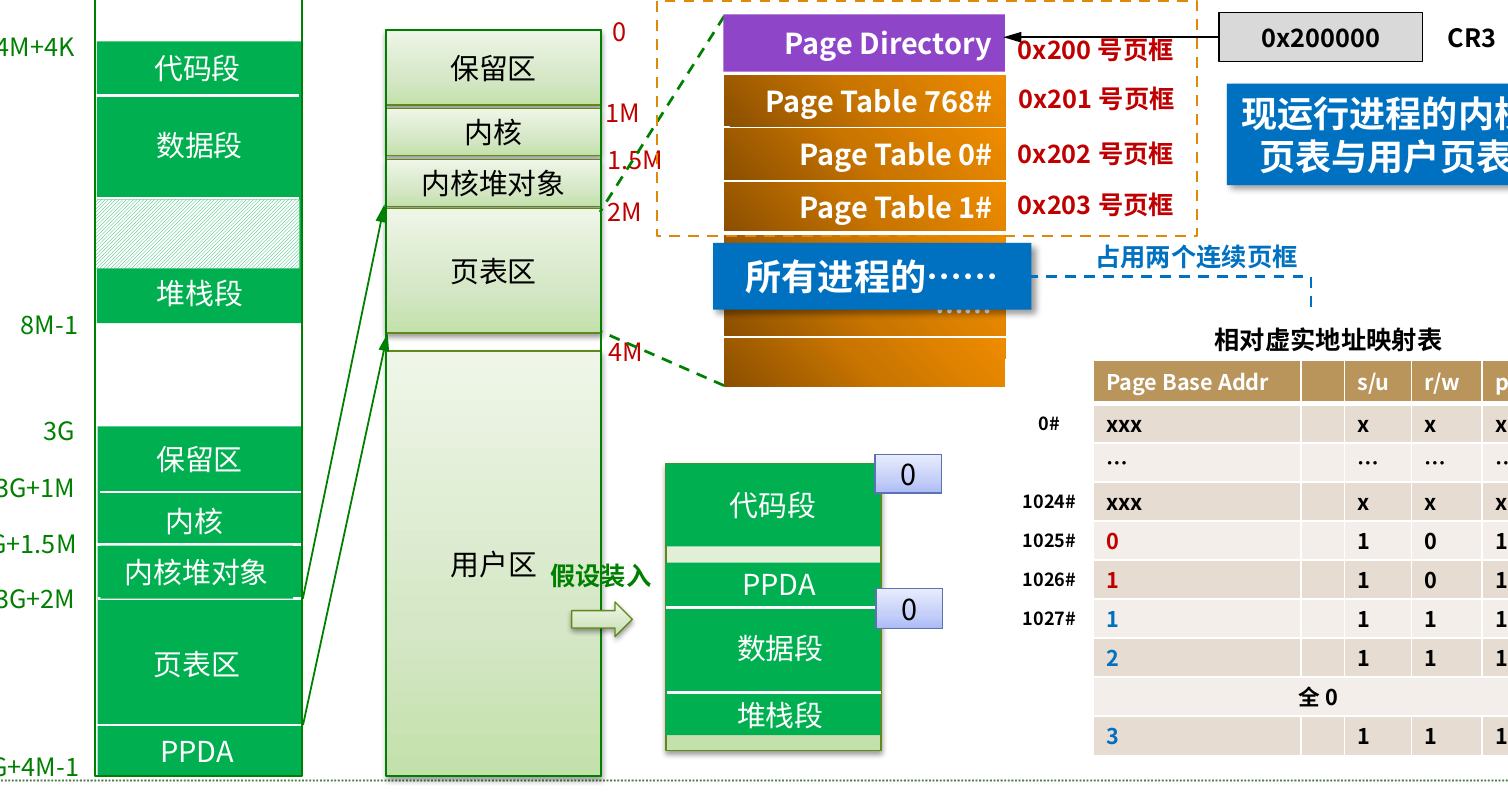
\includegraphics[width=0.9\textwidth]{figures/fig_pt_struct.png}
  \caption{页目录、页表与页框的构成关系（图源：课程设计 PPT slide 6）}
  \label{fig:pt-struct}
\end{figure}

在 80386 的两级页表机制下，一个页目录含 1024 个页目录项（PDE），每项指向一张页表；
一张页表含 1024 个页表项（PTE），每项映射一个 4KB 页框，故一张页表覆盖 4MB 虚拟
空间（\texttt{PageTable::SIZE\_PER\_PAGETABLE\_MAP = 0x400000}）。本设计中内核空间
固定从 \texttt{0xC0000000}（3G）起的 4MB，恰好对应页目录的第 768 项（
\texttt{0xC0000000 / 0x400000 = 768}）；用户空间从 0 起的 8MB 则由 0\# 与 1\# 两张
用户页表共同覆盖。

\section{内核页表与共享用户页表初始化}
并非所有页表都需要随进程切换。核心页表与 0\# 用户页表的内容对所有进程都相同，
因此被设计为\textbf{全局共享}，只在系统初始化时建立一次。\texttt{Machine} 类为此
新增了两个初始化接口（\texttt{Machine.h}，标注 NOTE 3）：

\begin{lstlisting}[caption={核心页表与共享用户页表的初始化接口},label={lst:machine-init}]
// 对应源码 include/Machine.h
void InitKernelPageTable();   // 初始化所有进程共享的核心页表(768#)
void InitZeroUserPageTable(); // 初始化所有进程共享的 0# 用户页表
\end{lstlisting}

其中，核心页表（768\#）把内核空间 \texttt{0xC0000000}\,–\,\texttt{0xC0400000} 恒等
映射到物理内存 \texttt{0x00000000}\,–\,\texttt{0x00400000}（即内核实际加载位置），
使得内核代码无论哪个进程运行都能被正确访问；0\# 用户页表则作为用户空间低 4MB 的
"共享窗口"，在 \texttt{exec} 构造参数栈时被临时借用（详见第五章）。

对于系统中的第一个进程——0\# 进程，其页目录在
\texttt{ProcessManager::SetupProcessZero()} 中被固定设置在页表区起始的物理页框上：

\begin{lstlisting}[caption={0\# 进程页目录的设置},label={lst:setup-zero}]
// 对应源码 proc/ProcessManager.cpp :: SetupProcessZero
pProcZero->pPageDirectory =
    (PageDirectory *)(Machine::PAGE_DIRECTORY_BASE_ADDRESS
                      + Machine::KERNEL_SPACE_START_ADDRESS);
// 物理地址 0x200000 + 虚地址偏移 0xC0000000 => 内核可访问的逻辑地址
\end{lstlisting}

注意此处把物理地址 \texttt{0x200000} 加上内核空间起始虚地址 \texttt{0xC0000000}，
得到内核视角下访问该页目录的逻辑地址——这正是核心页表恒等映射的用途。

\section{进程私有页目录与私有用户页表}
除共享部分外，每个进程还需要属于自己的页目录与一张私有 1\# 用户页表。为此，
\texttt{Process} 类新增了指向本进程页目录的指针及一个将其换算为物理地址的接口
（\texttt{include/Process.h}，标注 NOTE 3）：

\begin{lstlisting}[caption={Process 类新增的页目录成员},label={lst:proc-pdir}]
public:
    PageDirectory *pPageDirectory;          // 指向本进程页目录的逻辑地址
    unsigned long GetPageDirectoryPhyAddr();// 换算为物理地址, 供写入 CR3
\end{lstlisting}

\texttt{GetPageDirectoryPhyAddr()} 的实现十分直接——由于 \texttt{pPageDirectory}
保存的是内核空间逻辑地址，减去内核空间起始地址 \texttt{0xC0000000} 即得物理地址。

进程创建时，\texttt{ProcessManager} 提供两个辅助函数来建立私有页目录：
\texttt{AllocPageDirectory()} 从内核页框池分配一页作为页目录；
\texttt{InitProcPageDirectory()} 则把三类页表项填入新页目录——共享的 0\# 用户页表、
核心页表，以及本进程私有的 1\# 用户页表：

\begin{lstlisting}[caption={进程私有页目录的初始化},label={lst:init-pdir}]
// 对应源码 proc/ProcessManager.cpp :: InitProcPageDirectory
void ProcessManager::InitProcPageDirectory(Process *proc, PageTable *privateUsrPageTable)
{
    PageDirectory *pPageDirectory = proc->pPageDirectory;
    // (1) 共享的 0# 用户页表
    pPageDirectory->m_Entrys[0].m_UserSupervisor   = 1;
    pPageDirectory->m_Entrys[0].m_Present           = 1;
    pPageDirectory->m_Entrys[0].m_ReadWriter        = 1;
    pPageDirectory->m_Entrys[0].m_PageTableBaseAddress = Machine::USER_PAGE_TABLE_BASE_ADDRESS >> 12;
    // (2) 核心页表 (页目录第 768 项)
    unsigned int kPageTableIdx = Machine::KERNEL_SPACE_START_ADDRESS / PageTable::SIZE_PER_PAGETABLE_MAP;
    pPageDirectory->m_Entrys[kPageTableIdx].m_UserSupervisor = 0;   // 内核态
    pPageDirectory->m_Entrys[kPageTableIdx].m_Present          = 1;
    pPageDirectory->m_Entrys[kPageTableIdx].m_ReadWriter       = 1;
    pPageDirectory->m_Entrys[kPageTableIdx].m_PageTableBaseAddress = Machine::KERNEL_PAGE_TABLE_BASE_ADDRESS >> 12;
    // (3) 私有 1# 用户页表 (本进程独有)
    unsigned long phyFrame = ((unsigned long)privateUsrPageTable - Machine::KERNEL_SPACE_START_ADDRESS) >> 12;
    pPageDirectory->m_Entrys[1].m_PageTableBaseAddress = phyFrame;
    pPageDirectory->m_Entrys[1].m_UserSupervisor = 1;
    pPageDirectory->m_Entrys[1].m_Present          = 1;
    pPageDirectory->m_Entrys[1].m_ReadWriter       = 1;
}
\end{lstlisting}

\begin{figure}[H]
  \centering
  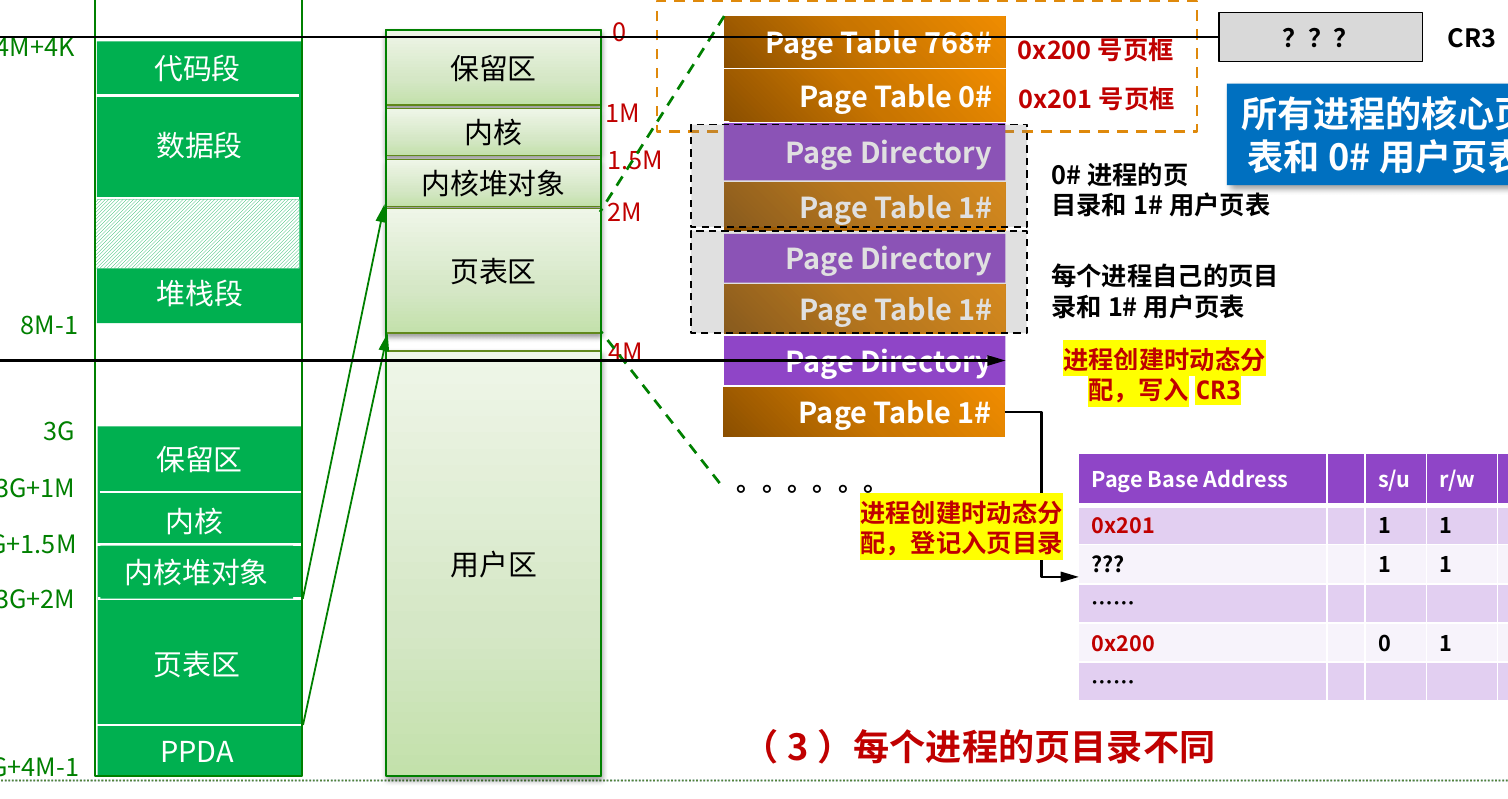
\includegraphics[width=0.85\textwidth]{figures/fig_private_pdir.png}
  \caption{每进程独立页目录与 CR3 的关系（图源：课程设计 PPT slide 10）}
  \label{fig:private-pdir}
\end{figure}

与每进程一张私有页目录相对应，\texttt{MemoryDescriptor} 也被简化为\textbf{只管理一页
私有用户页表}。\texttt{Initialize()} 只分配一页（而非原来的两张），
\texttt{Release()} 只回收一页，\texttt{ClearUserPageTable()} 只清除一页的表项。
这一变化是页表改造的直接结果：既然每进程只有一张私有用户页表（1\#），那么围绕它的
分配、回收与清零都自然以一页为单位。

\section{进程切换与 CR3 刷新}
页目录私有化之后，进程切换的核心动作就从"重写共享页表项"变成了"更换 \texttt{CR3}
指向目标进程的页目录"。这一变化集中体现在 \texttt{SwtchUStruct} 宏中：

\begin{lstlisting}[caption={进程切换宏 SwtchUStruct 的改造},label={lst:swtch}]
// 对应源码 (PPT slide 17)
#define SwtchUStruct(p)                                                         \
    Machine::Instance().GetKernelPageTable()                                    \
        .m_Entrys[Kernel::USER_PAGE_INDEX].m_PageBaseAddress = (p)->p_addr >> 12; \
    FlushPageDirectory((p)->GetPageDirectoryPhyAddr());
\end{lstlisting}

\begin{figure}[H]
  \centering
  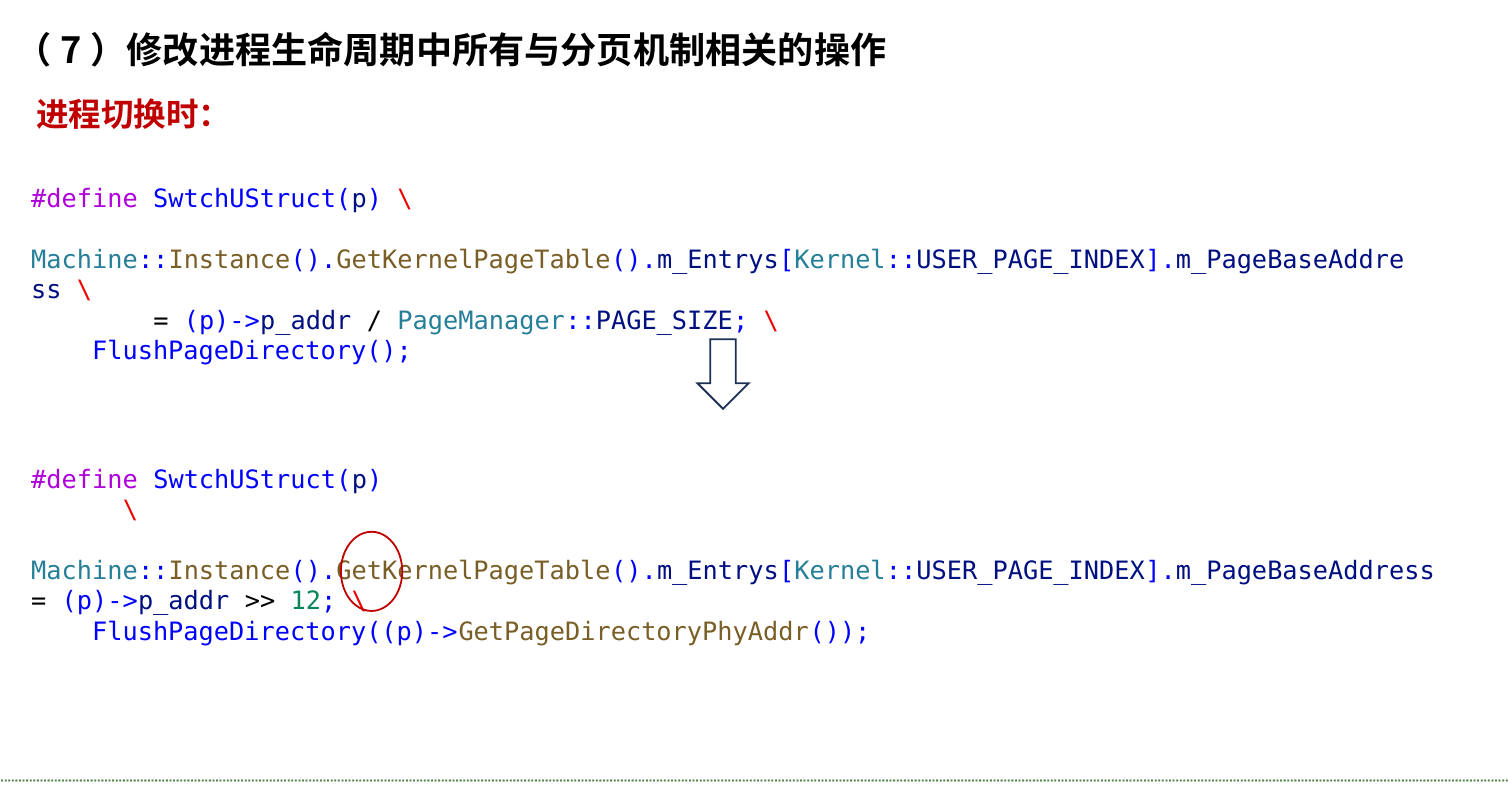
\includegraphics[width=0.85\textwidth]{figures/fig_swtch.png}
  \caption{进程切换宏 SwtchUStruct 的改造对比（图源：课程设计 PPT slide 17）}
  \label{fig:swtch}
\end{figure}

该宏完成两件事：其一，把核心页表中用于映射当前进程 user 结构（即 PPDA）的那一项，
更新为目标进程的 \texttt{p\_addr}（\texttt{Kernel::USER\_PAGE\_INDEX} 标识该 PTE 在
核心页表中的位置）；其二，调用 \texttt{FlushPageDirectory()} 把目标进程页目录的
物理地址写入 \texttt{CR3}，使新页目录立即生效。\texttt{FlushPageDirectory} 的实现
就是一条 \texttt{movl \%0, \%cr3} 指令。值得注意的是，与原系统固定刷新到
\texttt{0x200000} 不同，改造后的版本以目标进程的页目录物理地址为参数，这正是
"每进程独立页目录"在切换路径上的体现。

在进程管理器的 \texttt{Swtch()} 调度流程中，选中目标进程后还会调用
\texttt{MapToPageTable()}，其改造后实现同样只是调用
\texttt{FlushPageDirectory(u.u\_procp->GetPageDirectoryPhyAddr())}，确保当前
\texttt{CR3} 与 user 结构中记录的进程页目录保持一致。

\section{页表改造后的效果与边界}
经过上述改造，页表系统具备了如下能力：每个进程拥有独立的 4MB 用户空间映射
（由私有 1\# 用户页表决定），进程间地址空间相互隔离；进程切换不再重写页表项，
而是通过一次 \texttt{CR3} 写入完成；核心页表与 0\# 用户页表全局共享，避免了
冗余的初始化与切换开销。

同时也需明确改造的边界。\texttt{m\_UserPageTableArray} 仅指向一页私有用户页表，
因此凡涉及它的分配、回收、清除操作都以一页为单位——这与原系统两张用户页表的
做法不同，是页表布局变化带来的连带修改。此外，原系统中那些"与相对映射表设置物理
页表相关"的接口函数（如旧的 \texttt{MapEntry} 系列重载）在新模型下不再需要，
本次改造中已将其注释移除。这些边界修改为后续章节的位示图分配与进程映像管理奠定
了地址映射层面的基础。

\subsection*{运行验证}
页表系统改造完成后，内核能够正常引导启动并进入 shell。图~\ref{fig:run-shell-ch3}
为系统在 QEMU 下启动后进入 shell 提示符 \texttt{[/]\#}、并执行目录列出的画面，根
目录下可见 \texttt{dev}、\texttt{Shell.exe}、\texttt{etc}、\texttt{bin} 等条目。系统
能够启动并支撑 shell 运行，从运行层面验证了每进程独立页目录、核心页表恒等映射与
页目录初始化的正确性。

\begin{figure}[H]
  \centering
  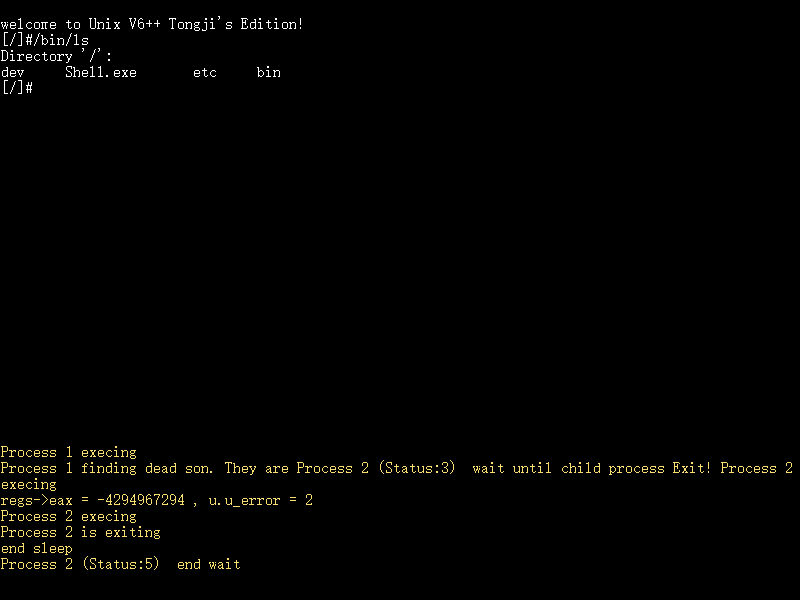
\includegraphics[width=0.85\textwidth]{figures/run_shell.png}
  \caption{页表系统改造后系统引导进入 shell}
  \label{fig:run-shell-ch3}
\end{figure}
    % 第三章  页表系统改造
% =====================================================================
%  第四章  物理页框分配方式改造
% =====================================================================
\chapter{物理页框分配方式改造}

\section{原 MapNode 连续空闲表分析}
页表系统改造完成后，下一个问题是物理页框的分配方式。原系统采用连续可变分区管理，
其核心数据结构是空闲分区表项 \texttt{MapNode}（\texttt{include/MapNode.h}）：

\begin{lstlisting}[caption={MapNode 空闲分区表项},label={lst:mapnode}]
struct MapNode
{
    unsigned long m_Size;       // 空闲分区大小 (页为单位)
    unsigned long m_AddressIdx; // 空闲分区起始地址
};
\end{lstlisting}

每个 \texttt{PageManager} 持有一张 \texttt{MapNode map[512]} 分区表，由
\texttt{Allocator::Alloc/Free}（对应 UNIX V6 的 \texttt{malloc/mfree}）维护：
\texttt{Alloc} 按首次适配找到第一块大小足够的分区，从其头部切出所需部分；
\texttt{Free} 则把释放的区域插回表中，并与前后相邻的空闲分区合并，以减少外部碎片。

这种连续分区方式有两个根本局限。其一，它要求被分配的区域在物理上\emph{连续}，
而页表改造后的离散化模型恰恰需要把一个进程的各虚页映射到\emph{任意}空闲物理页框，
连续性约束与之直接冲突。其二，连续分区在长期运行后难免产生外部碎片，即便总空闲量
充足也可能分配失败。因此，把物理页框的分配方式从连续分区改造为以单个页框为单位
的离散分配，就成了本次改造的第二块工作。

\begin{figure}[H]
  \centering
  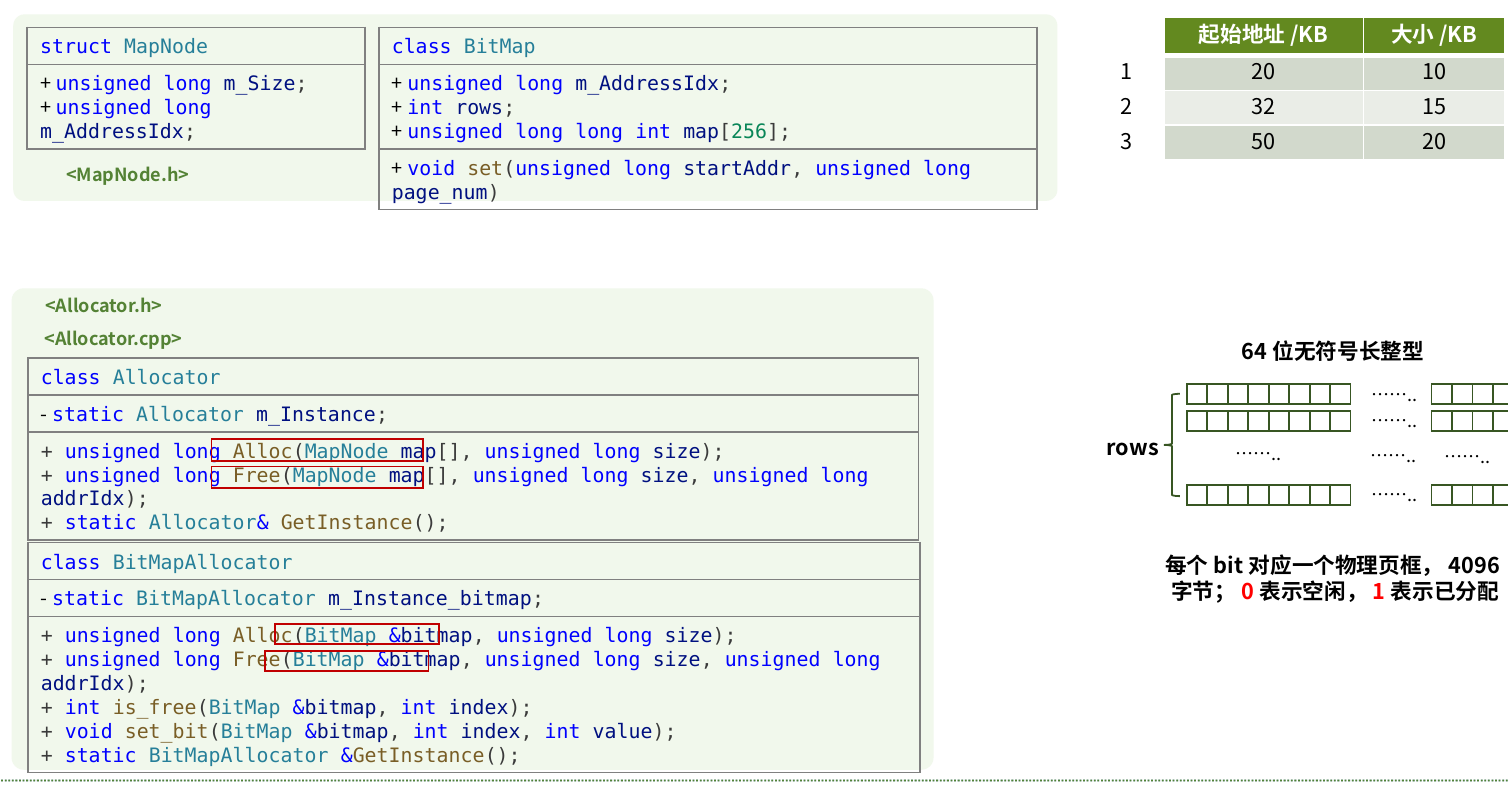
\includegraphics[width=0.9\textwidth]{figures/fig_bitmap_struct.png}
  \caption{从 MapNode 到 BitMap 的结构对比与位示图原理（图源：课程设计 PPT slide 23）}
  \label{fig:bitmap-struct}
\end{figure}

\section{bitmap 页框分配器设计}
本设计引入位示图（bitmap）作为新的页框管理结构。其核心思想是：用一个 bit 对应
一个 4KB 物理页框，0 表示空闲、1 表示已分配。由于不再要求连续，分配时只需在位示图
中找到足够数量的空闲 bit 即可，它们对应的物理页框不必相邻。\texttt{BitMap} 的定义
如下（\texttt{include/MapNode.h}，标注 NOTE 1）：

\begin{lstlisting}[caption={BitMap 位示图结构},label={lst:bitmap}]
#define M_PAGE_SIZE 4096
class BitMap
{
public:
    unsigned long m_AddressIdx;            // 本位示图管理的起始物理地址
    int rows;                              // 有效行数 (每行 64 bit)
    unsigned long long int map[256];        // 位示图本体, 256*64=16384 bit
    void set(unsigned long startAddr, unsigned long page_num)
    {
        m_AddressIdx = startAddr;
        rows = page_num / 64;
        for (int i = 0; i < rows; i++) map[i] = 0;   // 初始化为全空闲
    };
};
\end{lstlisting}

\begin{figure}[H]
  \centering
  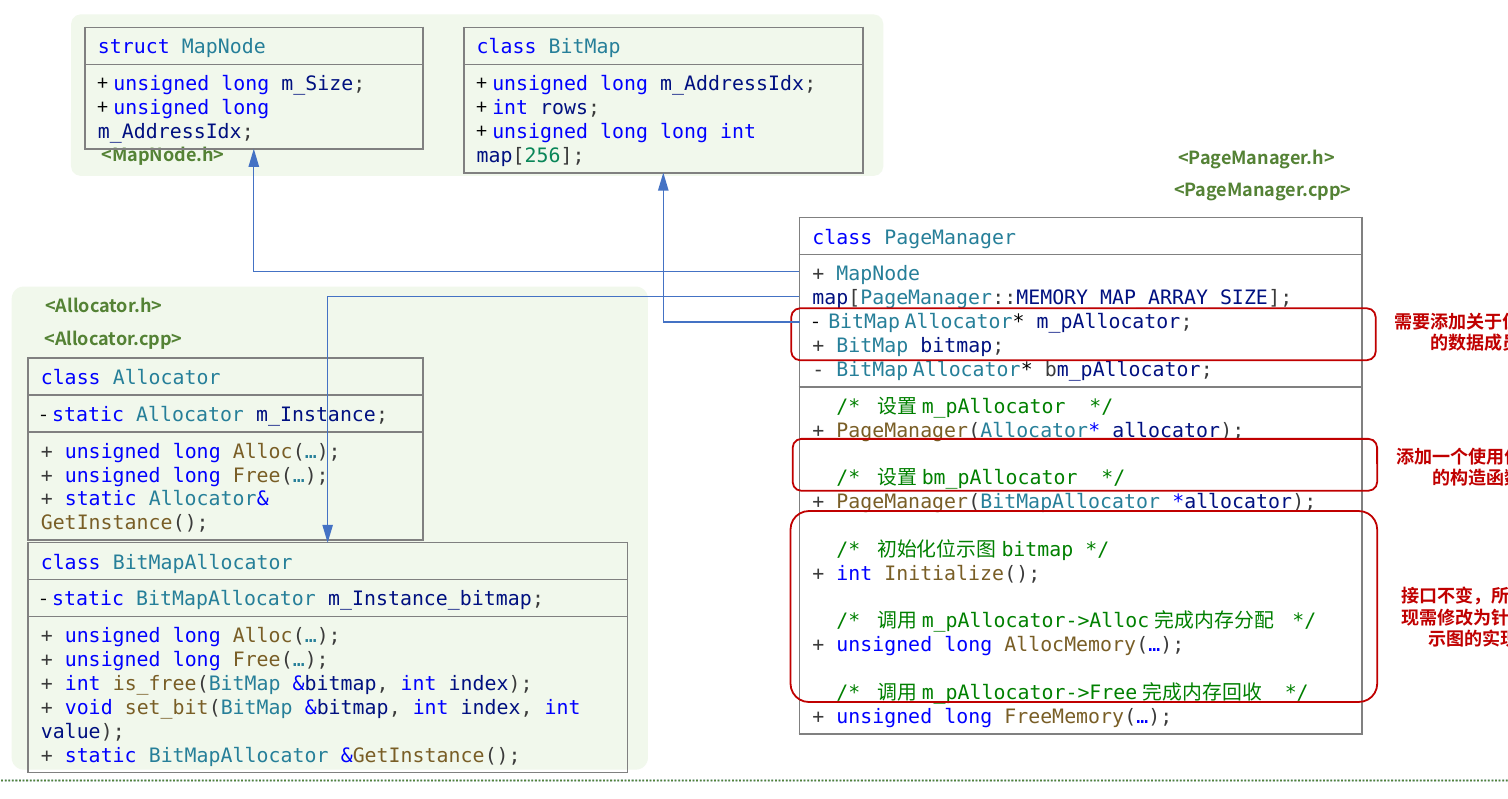
\includegraphics[width=0.9\textwidth]{figures/fig_bitmap_class.png}
  \caption{位示图管理相关的类与结构体关系（图源：课程设计 PPT slide 25）}
  \label{fig:bitmap-class}
\end{figure}

\texttt{map} 是一个 256 元素的 64 位无符号整数数组，共 $256\times 64 = 16384$ 个 bit，
最多可表示 16384 个页框，即 64MB 物理内存的页框占用情况（本设计 QEMU 配置 32MB
内存，容量充裕）。\texttt{m\_AddressIdx} 记录该位示图所管理区域的起始物理地址，
用于在位号与物理地址之间换算。

配套的分配器类 \texttt{BitMapAllocator}（\texttt{include/Allocator.h}）提供分配、
释放及位操作接口：

\begin{lstlisting}[caption={BitMapAllocator 接口},label={lst:bitmap-allocator-if}]
class BitMapAllocator
{
public:
    unsigned long Alloc(BitMap &bitmap, unsigned long size);
    unsigned long Free(BitMap &bitmap, unsigned long size, unsigned long addrIdx);
    int  is_free(BitMap &bitmap, int index);
    void set_bit(BitMap &bitmap, int index, int value);
    static BitMapAllocator &GetInstance();
};
\end{lstlisting}

\section{BitMapAllocator 的分配与释放}
\texttt{BitMapAllocator} 的分配算法在位示图中线性扫描，寻找一段连续的空闲 bit
（注意：这里要求的是\emph{位号连续}，对应物理页框在 bitmap 中编号连续，但由于
每页独立映射，物理页框是否相邻并不影响用户态连续性）。其实现见代码清单~%
\ref{lst:bitmap-alloc}。

\begin{lstlisting}[caption={BitMapAllocator::Alloc 分配算法},label={lst:bitmap-alloc}]
// 对应源码 mm/Allocator.cpp
unsigned long BitMapAllocator::Alloc(BitMap &bitmap, unsigned long size)
{
    int pages_needed = (size + M_PAGE_SIZE - 1) / M_PAGE_SIZE; // 向上取整所需页数
    int start = -1, count = 0;
    for (int i = 0; i < bitmap.rows * 64; i++)      // 扫描位示图
    {
        if (is_free(bitmap, i))                      // 第 i 位空闲
        {
            if (count == 0) start = i;               // 记录连续段起点
            if (++count == pages_needed) break;      // 找够所需页数
        }
        else count = 0;                              // 中断, 重新计数
    }
    if (count < pages_needed) return 0;              // 无足够空闲页
    for (int i = 0; i < pages_needed; i++)
        set_bit(bitmap, start + i, 1);               // 标记为已分配
    return start * M_PAGE_SIZE + bitmap.m_AddressIdx;// 返回起始物理地址
}
\end{lstlisting}

\texttt{Free} 是其逆过程：由释放地址反算起始位号，再把对应各位置 0。\texttt{is\_free}
与 \texttt{set\_bit} 是位运算原语，利用 64 位整数的位掩码完成单 bit 的读取与置位
（\texttt{map[index/64] \& (1ULL << (index\%64))}）。可以看到，整个分配器只依赖
位运算，不涉及分区表的插入、合并、搬移，实现简洁，且天然支持离散分配。

\section{内核页框池与用户页框池划分}
位示图建立之后，物理内存被划分为多个页框池，分别由不同的 \texttt{PageManager}
子类用各自的位示图管理。\texttt{PageManager}（\texttt{mm/PageManager.cpp}）在原有
\texttt{MapNode map[]} 的基础上新增了位示图成员 \texttt{bitmap} 与引用计数数组
\texttt{Page[]}，并增加了接受 \texttt{BitMapAllocator*} 的构造函数：

\begin{lstlisting}[caption={PageManager 新增的位示图与引用计数成员},label={lst:pm-members}]
// 对应源码 include/PageManager.h
class PageManager
{
public:
    MapNode map[PageManager::MEMORY_MAP_ARRAY_SIZE];
    BitMap bitmap;                                         // NOTE 1: 位示图
    int Page[MemoryDescriptor::USER_SPACE_SIZE / PAGE_SIZE]; // NOTE 3: 页引用计数
private:
    BitMapAllocator *m_pAllocator;
    unsigned long AllocMemory(unsigned long size);         // 调用 m_pAllocator->Alloc
    unsigned long FreeMemory(unsigned long size, unsigned long startAddress);
};
\end{lstlisting}

两个子类分别划定各自的管理范围。\texttt{KernelPageManager} 管理页表区中除固定占用
部分（页目录、核心页表、0\# 用户页表共占 4 页）之外的剩余页框，其起始地址定义为
\texttt{0x200000 + 0x2000 + 0x2000 = 0x204000}，大小为
\texttt{0x200000 - 0x4000}；\texttt{UserPageManager} 则管理从 \texttt{0x400000}
（4M）起至整个物理内存末端的用户区。两者在 \texttt{Initialize()} 中分别调用
\texttt{bitmap.set(...)} 把各自范围初始化为全空闲：

\begin{lstlisting}[caption={用户页框池的位示图初始化},label={lst:user-pm-init}]
// 对应源码 mm/PageManager.cpp :: UserPageManager::Initialize
this->map[0].m_AddressIdx = USER_PAGE_POOL_START_ADDR / PageManager::PAGE_SIZE;
this->map[0].m_Size       = USER_PAGE_POOL_SIZE / PageManager::PAGE_SIZE;
this->bitmap.set(USER_PAGE_POOL_START_ADDR, USER_PAGE_POOL_SIZE / PageManager::PAGE_SIZE);
\end{lstlisting}

需要强调的是，bitmap 只管理"可动态分配"的页框池；内核映像本身、页目录及固定页表
所占用的页框是静态固定的，不在 bitmap 的动态分配范围之内，因此不会与之冲突。

\section{页引用计数机制}
仅有位示图还不够。写时复制（COW）与正文段共享都允许多个进程的页表项指向同一个
物理页框，因此一个物理页是否能够真正释放，不能只看某一个页表项，而要看它是否还被
其他进程引用。为此，\texttt{PageManager} 引入了页引用计数数组 \texttt{Page[]}，
其长度为用户空间大小除以页大小（\texttt{USER\_SPACE\_SIZE / PAGE\_SIZE}），
\texttt{Page[i]} 记录第 \texttt{i} 个用户区物理页框的共享份数。

引用计数与分配、释放逻辑紧密耦合（\texttt{mm/PageManager.cpp}）：

\begin{lstlisting}[caption={带引用计数的分配与释放},label={lst:page-refcount}]
unsigned long PageManager::AllocMemory(unsigned long size)
{
    unsigned long newaddr = this->m_pAllocator->Alloc(this->bitmap, size);
    Page[newaddr >> 12] = 1;                       // 新分配页, 引用计数置 1
    return newaddr;
}
unsigned long PageManager::FreeMemory(unsigned long size, unsigned long startAddress)
{
    Page[startAddress >> 12]--;                     // 引用计数减一
    if (Page[startAddress >> 12] == 0)              // 无人再引用, 才真正释放
        this->m_pAllocator->Free(this->bitmap, size, startAddress);
    return 1;
}
\end{lstlisting}

\texttt{AllocMemory} 在分配后立即把对应页的引用计数置为 1；\texttt{FreeMemory}
则\emph{先}把引用计数减一，只有当计数归零时才调用底层的 \texttt{BitMapAllocator::Free}
真正归还页框。配合 \texttt{fork} 时对共享页的 \texttt{Page[]++}（见第五章），物理页的
生命周期便由引用计数而非单个页表项统一管理，这正是 COW 与 text 共享得以正确释放的
关键。

\section{KernelAllocator 的同步适配}
值得说明的是，位示图改造集中在 \texttt{PageManager} 体系（页表区与用户区），而
管理内核堆对象区的 \texttt{KernelAllocator} 仍沿用原有的连续分区方式——它依旧
持有 \texttt{MapNode map[]} 并通过旧的 \texttt{Allocator::Alloc/Free} 进行分配，
管理从 \texttt{0x180000}（1.5M）起的 512KB 内核堆（\texttt{include/KernelAllocator.h}）。

这一"不改"本身就是一种经过权衡的取舍：内核堆对象多为变长的小对象（如各种内核数据
结构的动态实例），连续分区的变长分配对这类场景更为合适；而位示图以页框为最小单位，
更适合页表、用户图像这类按页分配的对象。因此本设计让两者并存：\texttt{KernelAllocator}
保持兼容以服务内核堆，\texttt{KernelPageManager}/\texttt{UserPageManager} 则全面转向
位示图以服务页框级分配。这种分工使得改造得以聚焦于真正需要离散化的部分，避免对内核
堆对象管理做不必要的、风险更高的改动。

\subsection*{运行验证}
为验证位示图分配在运行时的正确性，在 shell 中执行 \texttt{/bin/malloc} 与
\texttt{/bin/stack} 两个用户程序。\texttt{malloc} 输出 \texttt{test of malloc}，
表明用户态堆分配（经内核堆对象区的分配管理）正常工作（图~\ref{fig:run-malloc}）；
\texttt{stack} 程序递归压栈、输出由大到小的计数，验证了离散页表下栈页能够按需扩展
分配（图~\ref{fig:run-stack}）。两者共同说明位示图分配能够支撑用户态堆栈的动态增长。

\begin{figure}[H]
  \centering
  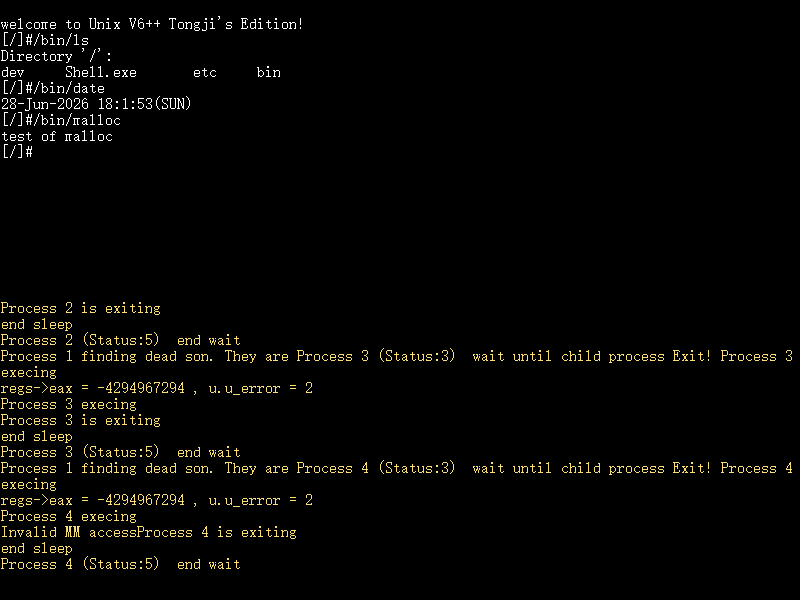
\includegraphics[width=0.85\textwidth]{figures/run_malloc.png}
  \caption{运行 /bin/malloc：用户堆分配测试}
  \label{fig:run-malloc}
\end{figure}

\begin{figure}[H]
  \centering
  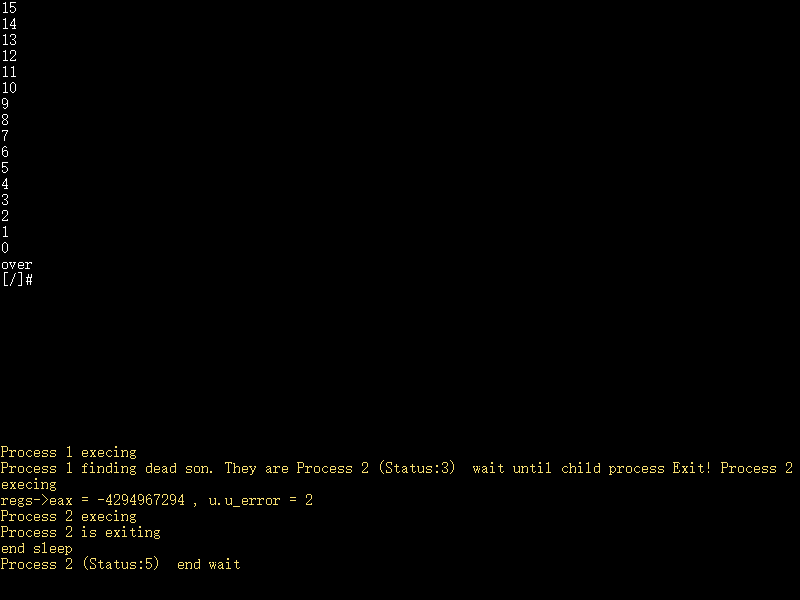
\includegraphics[width=0.85\textwidth]{figures/run_stack.png}
  \caption{运行 /bin/stack：离散页表下栈按需扩展}
  \label{fig:run-stack}
\end{figure}

\section{本章小结}
本章把物理页框的分配方式从连续空闲分区表改造为位示图。\texttt{BitMap} 以每页一个
bit 的粒度记录页框占用，\texttt{BitMapAllocator} 通过位运算完成离散分配与释放；
页表区与用户区分别由 \texttt{KernelPageManager}/\texttt{UserPageManager} 用各自的
位示图管理；\texttt{Page[]} 引用计数则与分配/释放逻辑耦合，为共享物理页的生命周期
管理提供依据。这一层改造与第三章的页表改造共同构成了离散化进程映像管理的物理基础。
    % 第四章  物理页框分配方式改造
% =====================================================================
%  第五章  离散化进程映像管理
% =====================================================================
\chapter{离散化进程映像管理}

\section{用户进程地址空间布局}
在新的页表与位示图基础设施之上，本章讨论进程映像在生命周期各关键时刻的管理。
首先要明确的是用户进程的地址空间布局。

尽管物理页框已经离散化，但\textbf{对用户程序而言，虚地址空间仍是连续的}：每个
用户进程拥有从 0 起的 8MB 虚拟空间（\texttt{MemoryDescriptor::USER\_SPACE\_SIZE
= 0x800000}），其中依次为代码段（text）、数据段（data）、堆（heap，向上扩展）与
栈（stack，自 8MB 顶端向下扩展）。这一布局与原系统保持一致，使得用户程序无需感知
物理页框是否连续——这正是分页机制"用页表把离散物理页拼接成连续虚拟空间"的核心价值，
也符合课设"离散化存储"的目标。

用户空间的映射由本进程私有的 1\# 用户页表承担。由于 0\# 用户页表覆盖低 4MB、1\#
用户页表覆盖高 4MB，而本设计中用户图像通常落在 1\# 页表管理的范围，因此在代码中
频繁出现如下页表下标换算：

\begin{lstlisting}[caption={用户虚地址到 1\# 页表项下标的换算},label={lst:pte-idx}]
// 虚地址 cr2 对应的 1# 用户页表项下标
unsigned int physicalBase =
    md.m_UserPageTableArray->m_Entrys[(cr2 >> 12) - 1024].m_PageBaseAddress;
\end{lstlisting}

\begin{figure}[H]
  \centering
  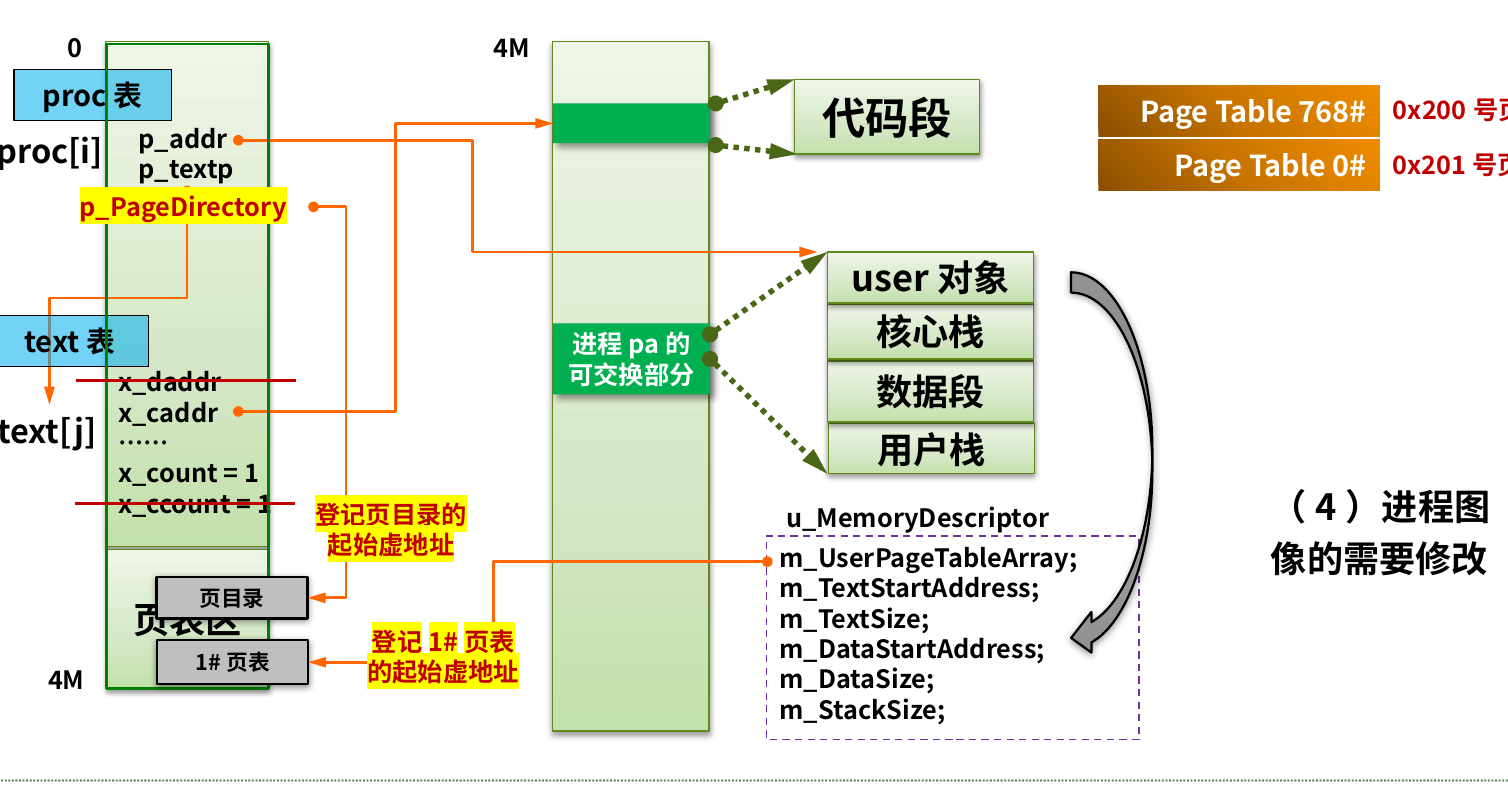
\includegraphics[width=0.9\textwidth]{figures/fig_proc_image.png}
  \caption{进程映像与页目录、页表、proc/text 表的关系（图源：课程设计 PPT slide 12）}
  \label{fig:proc-image}
\end{figure}

其中 \texttt{(cr2 >> 12)} 得到虚页号，减去 1024（即一张页表的表项数）是为了从 1\#
页表的角度换算下标——这一"减 1024"的约定贯穿了 fork、缺页、exec 等所有涉及用户页表
操作的路径。

\section{fork 与 COW 建立}
\texttt{fork} 是离散化改造中变化最大的路径之一。改造后的 \texttt{NewProc()} 不再
整体复制父进程图像，而是为子进程建立一套独立的页表结构，并与父进程\emph{共享}物理
页（写时复制）。其核心流程见代码清单~\ref{lst:newproc}。

\begin{lstlisting}[caption={fork (NewProc) 的 COW 建立},label={lst:newproc}]
// 对应源码 proc/ProcessManager.cpp :: NewProc
// NOTE 3: 为子进程建立私有页表与页目录
u.u_MemoryDescriptor.Initialize();                       // 分配子进程私有 1# 用户页表
PageTable *desPgTable = u.u_MemoryDescriptor.m_UserPageTableArray;
child->pPageDirectory   = ProcessManager::AllocPageDirectory(); // 子进程页目录
ProcessManager::InitProcPageDirectory(child, desPgTable);        // 填写页目录

// NOTE 4: 为子进程 PPDA 分配一页, 复制父进程 PPDA
unsigned long desAddress = userPageManager.AllocMemory(PageManager::PAGE_SIZE);
child->p_addr = desAddress;
Utility::CopySeg(current->p_addr, desAddress);

// NOTE 5 + COW: 复制父进程 1# 用户页表, 并把共享页置只读、引用计数加一
if (pgTable) {
    ProcessManager::ModifyPageTable(userPageManager, pgTable);   // 置 RW=0, Page[]++
    Utility::MemCopy((unsigned long)pgTable, (unsigned long)desPgTable, sizeof(PageTable));
}
\end{lstlisting}

其中 \texttt{ModifyPageTable()} 是 COW 建立的关键：它遍历父进程页表中所有"已存在且
可写"的表项，将其读写位 \texttt{m\_ReadWriter} 改为 0（只读），并对这些表项指向的
物理页框把引用计数 \texttt{Page[]} 加一：

\begin{lstlisting}[caption={ModifyPageTable: 共享页置只读并增加引用计数},label={lst:modify-pt}]
// 对应源码 proc/ProcessManager.cpp :: ModifyPageTable
void ProcessManager::ModifyPageTable(UserPageManager &userPageManager, PageTable* pgTable) {
    for (unsigned int j = 0; j < PageTable::ENTRY_CNT_PER_PAGETABLE; j++) {
        if (pgTable->m_Entrys[j].m_Present && pgTable->m_Entrys[j].m_ReadWriter) {
            pgTable->m_Entrys[j].m_ReadWriter = 0;                       // 置只读
            userPageManager.Page[pgTable->m_Entrys[j].m_PageBaseAddress]++; // 引用计数++
        }
    }
}
\end{lstlisting}

随后，父进程的整张 1\# 用户页表被原样复制给子进程（\texttt{MemCopy}）。于是 fork
完成后，父子两进程的页表完全相同，都把各自的数据/栈虚页指向\emph{同一批}物理页框，
且这些页框的页表项都被标记为只读、引用计数为 2。此时并没有发生任何用户图像的复制
（仅复制了页表这一页本身），这正是"写时复制"中"写时"之前的状态。

\section{page fault 中的 COW 处理}
COW 的真正复制发生在某一方尝试写入共享只读页时——这会触发缺页异常
（page fault），由 \texttt{Exception::PageFault()} 统一处理。该函数读取 \texttt{CR2}
得到缺页虚地址，判断这是否是一次"写只读共享页"的 COW 请求，并据此决定是直接放开
写权限还是复制新页，见代码清单~\ref{lst:cow-fault}。

\begin{lstlisting}[caption={page fault 中的 COW 处理},label={lst:cow-fault}]
// 对应源码 interrupt/Exception.cpp :: PageFault (节选)
unsigned char RW = md.m_UserPageTableArray->m_Entrys[(cr2 >> 12) - 1024].m_ReadWriter;
bool isRW = (cr2 >= md.m_DataStartAddress && cr2 < md.m_DataStartAddress + md.m_DataSize)
         || (cr2 >= USER_SPACE_SIZE - md.m_StackSize && cr2 < USER_SPACE_SIZE);
unsigned int physicalBase = md.m_UserPageTableArray->m_Entrys[(cr2 >> 12) - 1024].m_PageBaseAddress;

if (RW == 0 && userPageMgr.Page[physicalBase] >= 1 && isRW)   // 只读共享页 + 写数据/栈
{
    if (userPageMgr.Page[physicalBase] == 1) {                 // 仅本进程持有
        md.m_UserPageTableArray->m_Entrys[(cr2 >> 12) - 1024].m_ReadWriter = 1; // 直接放开写
        return;
    } else {                                                   // 还被其他进程共享
        --userPageMgr.Page[physicalBase];                      // 引用计数减一
        unsigned long newPage = userPageMgr.AllocMemory(M_PAGE_SIZE); // 分配新页
        md.m_UserPageTableArray->m_Entrys[(cr2 >> 12) - 1024].m_PageBaseAddress = newPage >> 12;
        md.m_UserPageTableArray->m_Entrys[(cr2 >> 12) - 1024].m_ReadWriter = 1; // 可写
        userPageMgr.Page[newPage >> 12] = 1;                   // 新页引用计数置 1
        Utility::CopySeg(physicalBase << 12, newPage);         // 复制原页内容
        return;
    }
}
\end{lstlisting}

这里体现了 COW 的两个分支。当 \texttt{Page[physicalBase] == 1} 时，说明该物理页虽然
被标记为只读共享，但实际上只剩当前进程一个引用者（其他进程已先后触发 COW 分离），
此时无需复制，直接把页表项的读写位置 1 即可；当 \texttt{Page[physicalBase] > 1} 时，
该页仍被其他进程共享，当前进程必须分配一个新物理页、复制原页内容、把页表项重定向到
新页，并把原页的引用计数减一。\texttt{isRW} 的判断确保只有对数据段或栈段的写入才走
COW 路径——代码段（text）本身就该只读共享，其写入应被视为非法访问。

若缺页既非 COW 请求、也非合法的栈扩展，则按非法内存访问处理：用户态越界发送
\texttt{SIGSEGV} 信号，内核态则 \texttt{Panic}。

\section{exec 图像改换与参数栈构造}
\texttt{exec} 是另一条高度改造的路径。原系统 \texttt{exec} 需要把新程序图像搬运到
一段连续的用户内存；改造后，本设计为\emph{新用户栈}分配物理页框，在其上接纳命令行
参数，然后直接建立用户页表映射，\emph{省去了整段图像的内存复制}。

\texttt{Exec()} 的参数栈构造是其精巧之处。由于用户程序尚未运行、其私有页表还未建立，
代码\emph{借用}全局共享的 0\# 用户页表作为临时窗口：先为新栈分配连续物理页框
（\texttt{trueStack}），把它们临时挂到 0\# 页表的前几项，使内核能通过低地址访问到
这些栈页；随后自顶向下在栈上依次写入命令行字符串、\texttt{argv[]} 指针数组、结束标志
与 \texttt{argc}；最后撤销对 0\# 页表的临时借用，恢复其原貌。关键代码见清单~%
\ref{lst:exec-stack}。

\begin{lstlisting}[caption={exec 借用 0\# 页表构造参数栈},label={lst:exec-stack}]
// 对应源码 proc/ProcessManager.cpp :: Exec (节选)
int pages = (parser.StackSize + PAGE_SIZE - 1) >> 12;
unsigned long trueStack = (userPgMgr.AllocMemory(pages << 12)) >> 12; // 为新栈分配物理页框
PageTableEntry *tempEntrys = (PageTableEntry *)Machine::Instance().GetUserPageTableArray();
for (int i = 1; i <= pages; i++, trueStack++) {           // 临时挂到 0# 页表
    tempEntrys[i].m_Present = 1; tempEntrys[i].m_ReadWriter = true;
    tempEntrys[i].m_PageBaseAddress = trueStack;
}
u.u_MemoryDescriptor.MapToPageTable();                    // 刷新使映射生效
// ... 自顶向下写入 argv 字符串、argv[] 指针数组、argc ...
for (int i = 1; i <= pages; i++) {                        // 恢复 0# 页表, 撤销借用
    tempEntrys[i].m_Present = 0; tempEntrys[i].m_ReadWriter = false;
}
u.u_MemoryDescriptor.MapToPageTable();
\end{lstlisting}

参数栈构造完成后，\texttt{Exec} 释放旧的正文段（\texttt{XFree}）、数据段与栈段，
再按 PE 文件头给出的新 \texttt{text}/\texttt{data}/\texttt{stack} 尺寸，分别为数据段、
栈段分配物理页框并填写私有 1\# 用户页表项；正文段则走共享路径（见下文）。最终通过
\texttt{Relocate} 完成重定位，并把返回地址设为程序入口，使系统调用返回 ring3 后从
新程序开始执行。整个过程中，用户图像不需要被整体搬运，仅需写入命令行参数与建立
页表映射。

\section{exit 与共享 text 释放}
进程退出时，需要释放其占用的物理页框。数据段与栈段页框由引用计数
（\texttt{Page[]--}）配合 \texttt{FreeMemory} 释放；而正文段由于可能被多个进程共享，
其释放由 \texttt{Text} 结构中的两个计数器控制（\texttt{proc/Text.cpp}）：

\begin{itemize}
  \item \texttt{x\_ccount}：当前在内存中（已加载）引用该正文段的进程数；
  \item \texttt{x\_count}：总体（含潜在换出）引用该正文段的进程数。
\end{itemize}

\texttt{Text::XccDec()} 在每次退出时被调用，先递减 \texttt{x\_ccount}，只有当它降到
0（即内存中已无进程使用该正文段）时，才真正释放正文段各页的物理页框；\texttt{XFree()}
则在 \texttt{XccDec} 基础上进一步判断 \texttt{x\_count}，当它也降为 0 时释放对应的
swap 副本与 inode。这种双层计数保证了正文段的物理页只在\emph{所有}共享者都退出后才
被回收，避免误释放仍被他进程使用的代码页。

\section{wait 写 status 时的 COW 处理}
父进程通过 \texttt{wait} 回收子进程时，往往需要把子进程的退出状态写入子进程的用户
地址空间。若该目标页恰好是 fork 时建立的 COW 共享只读页，这一写入会自然地触发缺页
异常，进而走与第 5.3 节完全相同的 COW 处理路径：分配新页、复制内容、重定向页表项。

也就是说，COW 机制并不专属于某一条系统调用，而是由 \texttt{PageFault} 统一兜底——
任何对只读共享页的写入，无论来自 fork 后的父子、wait 的状态写回，还是其他路径，都会
被同一套引用计数判断与复制逻辑接管。这种"机制统一、调用无关"的设计，使得 COW 能够
一致地覆盖进程生命周期中所有涉及共享页写入的场景。需要指出的是，COW 判断的地址范围
（\texttt{isRW}）必须准确覆盖数据段与栈段，否则会出现共享页无法及时分离的问题，
这一点将在第七章 7.2 节作为一个实际调试案例讨论。

\section{堆扩展与栈扩展}
离散化模型下，堆与栈的动态扩展变得十分自然。\texttt{SBreak}（响应 \texttt{brk}
系统调用）扩展堆时，只需为新虚页分配空闲物理页框并在私有页表中建立映射，无需像
连续模型那样保证与既有区域物理相邻；\texttt{SStack} 处理栈的自动向下扩展——当访问
超越当前栈顶但仍在合理范围内的地址时，\texttt{PageFault} 会判定为合法的栈扩展
（见第 5.3 节末尾的栈扩展分支），调用 \texttt{SStack} 补齐缺失的栈页。

由于每次扩展都只涉及"分配新页框 + 更新私有页表项"两步，不依赖连续物理内存，离散化
模型从根本上消除了原连续模型下扩展可能因找不到连续区而失败的问题，也为按需分配
（demand paging）提供了天然支持。

\subsection*{运行验证}
执行 \texttt{/bin/echo hello}，程序正确输出参数 \texttt{hello}（图~\ref{fig:run-echo}），
验证了 \texttt{exec} 借用 0\# 页表构造参数栈、向新程序传递 \texttt{argc}/\texttt{argv}
的机制。执行 \texttt{/bin/forks}，程序连续 \texttt{fork} 创建多个子进程（PID 依次
递增），父进程经 \texttt{wait} 逐个回收（图~\ref{fig:run-forks}），验证了 fork 写时
复制建立共享页、进程映像离散存放与按引用回收在多次进程创建下的正确性。

\begin{figure}[H]
  \centering
  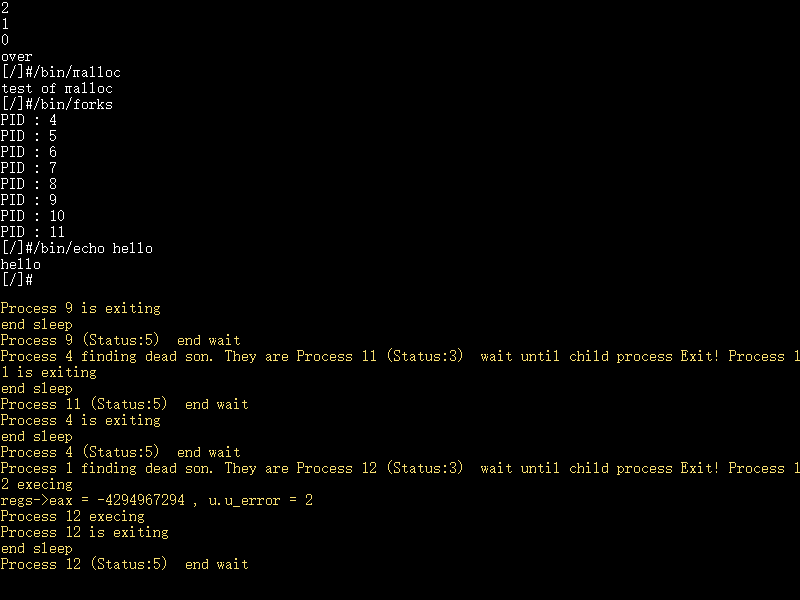
\includegraphics[width=0.85\textwidth]{figures/run_echo.png}
  \caption{运行 /bin/echo hello：exec 命令行参数传递验证}
  \label{fig:run-echo}
\end{figure}

\begin{figure}[H]
  \centering
  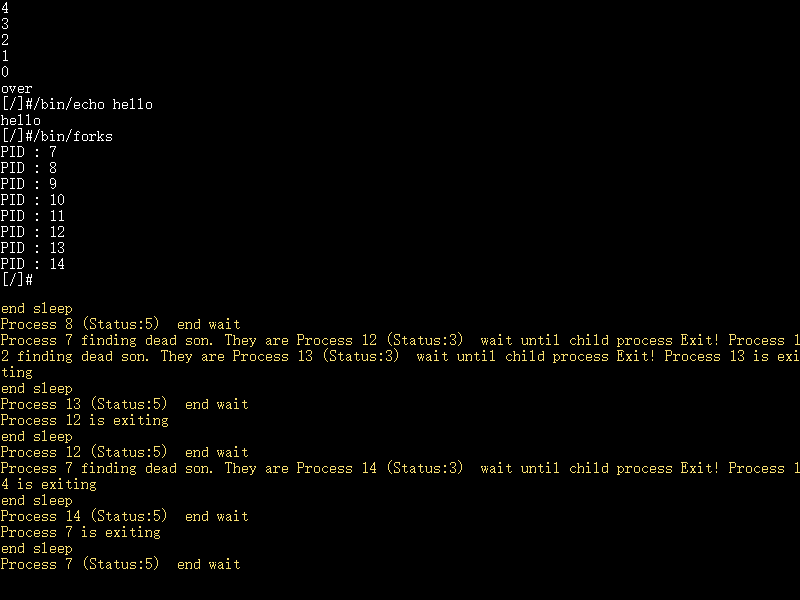
\includegraphics[width=0.85\textwidth]{figures/run_forks.png}
  \caption{运行 /bin/forks：多进程创建与进程映像离散化验证}
  \label{fig:run-forks}
\end{figure}

\section{本章小结}
本章把进程映像管理全面转向离散模型：fork 用 COW 延迟复制，仅在真正写入时经
\texttt{PageFault} 分离共享页；exec 用借用 0\# 页表构造参数栈、直接挂用户页表，省去
图像搬运；text 段用 \texttt{x\_ccount}/\texttt{x\_count} 双计数实现共享与按引用释放；
堆栈扩展则降级为"分配页框 + 更新页表"。配合第四章的位示图与引用计数，物理页的生命
周期得以由共享语义而非单个页表项正确管理，"离散存放 + 按需分配"的进程映像管理目标
至此基本达成。
        % 第五章  离散化进程映像管理
% =====================================================================
%  第六章  本地运行环境与工程适配
% =====================================================================
\chapter{本地运行环境与工程适配}

\section{Windows/MSYS2/MinGW 构建环境}
UNIX V6++ 原生面向 Windows 平台，其工具链由 MSYS2/MinGW 提供。具体包括：汇编器
NASM 用于引导与第二阶段加载代码；编译器 g++（内核）/ gcc（用户程序）以
freestanding 方式工作，关闭标准库与运行时（\texttt{-nostdlib -nostartfiles
-fno-builtin -fno-rtti -fno-exceptions -nostdinc}）；链接器 ld 按自定义脚本
\texttt{Link.ld} 链接，输出格式为 \texttt{pei-i386}；\texttt{objcopy}/
\texttt{objdump}/\texttt{nm} 用于把可链接映像转为裸二进制并生成符号表与反汇编。
运行环境则使用 Bochs 或 QEMU（\texttt{qemu-system-i386}）加载磁盘镜像验证。

本设计的本地验证在 Linux 环境下进行，其工具链与 Windows 版高度等价：系统自带的
\texttt{gcc/g++} 经 \texttt{-m32} 即可生成 32 位代码，binutils 的 \texttt{ld} 同样
支持 \texttt{pei-i386} 输出格式，\texttt{objcopy}/\texttt{objdump}/\texttt{nm} 均已
就绪；仅需额外安装 \texttt{nasm}（汇编）与 \texttt{qemu-system-i386}（运行）。
内核链接得到的 \texttt{kernel.exe} 与在 Windows 下产物一致，可直接进入后续镜像
构建流程。

\section{Makefile 与构建流程适配}
工程的构建由分层的 Makefile 组织。顶层 \texttt{Makefile} 通过 \texttt{include
Makefile.inc} 定义公共变量与规则，再以 \texttt{DIRS} 列表递归进入各子目录
（\texttt{boot}、\texttt{kernel}、\texttt{mm}、\texttt{proc}、\texttt{interrupt}、
\texttt{fs}、\texttt{dev} 等）分别编译，最终在 \texttt{build} 目标中完成链接与转换：

\begin{lstlisting}[caption={内核构建的核心步骤},label={lst:build}]
# 对应源码 Makefile (build 目标, 改写为跨平台等价命令)
$(LD) $(LDFLAGS) $(OBJS) -o kernel.exe        # 链接为 PE 可执行
objcopy -O binary kernel.exe kernel.bin         # 转为裸二进制
nm      kernel.exe > kernel.sym                 # 符号表 (调试用)
objdump -d     kernel.exe > kernel.asm          # 反汇编 (调试用)
\end{lstlisting}

链接脚本 \texttt{Link.ld} 规定了内核的内存布局（见代码清单~\ref{lst:linkld}）：
入口符号为 \texttt{greatstart}；\texttt{.text} 段定位于 \texttt{0xc0100000}（即内核
空间 \texttt{0xC0000000} 偏上 1MB 处），其后依次为 \texttt{.data}（含构造/析构表）与
\texttt{.bss}，各段按 4KB 对齐。这一布局与第三章中核心页表把 \texttt{0xC0000000} 起
4MB 恒等映射到物理低址的设计相吻合——内核被 bootloader 加载到物理 1MB 处后，即可
通过该恒等映射在 \texttt{0xc0100000} 虚地址上正确执行。

\begin{lstlisting}[caption={Link.ld 的关键约束},label={lst:linkld}]
/* 对应源码 Link.ld */
OUTPUT_FORMAT("pei-i386")
ENTRY(greatstart)
SECTIONS {
    .text 0xc0100000 : { *(.text) . = ALIGN(4096); }
    .data : { /* .ctors / .dtors 构造析构表 */ *(.data) . = ALIGN(4096); }
    .bss  : { *(.bss)  . = ALIGN(4096); }
}
\end{lstlisting}

由于原 Makefile 大量使用 Windows 专有命令（\texttt{copy}/\texttt{del}、反斜杠路径），
本地适配时需要将这些命令替换为跨平台等价形式（\texttt{cp}/\texttt{rm}、正斜杠路径），
或直接在 MSYS2 环境下沿用原版。这一适配不涉及算法逻辑，但直接影响构建能否走通。

\section{bootloader 与内核镜像适配}
系统启动由 \texttt{boot.s} 完成。它是一段仅 512 字节的引导扇区，承担从 16 位实模式
进入 32 位保护模式并加载内核的职责，其流程为：加载 GDT、开启 A20 地址线、置
\texttt{CR0} 的 PE 位进入保护模式、远跳转到 32 位代码段；随后以 LBA28 PIO 方式从硬盘
读取内核映像到物理地址 \texttt{0x100000}（1MB），读取的扇区数由 \texttt{KERNEL\_SIZE}
决定；最后切换数据段、把 \texttt{esp} 或上 \texttt{0xc0000000} 转入内核虚地址视角，
远跳转到 \texttt{0xc0100000} 开始执行内核入口。关键代码见清单~\ref{lst:boot}。

\begin{lstlisting}[caption={boot.s 加载内核的核心逻辑},label={lst:boot}]
; 对应源码 boot/boot.s (32 位段节选)
mov  ecx, KERNEL_SIZE        ; 要加载的扇区数
mov  eax, 1                  ; LBA 起始扇区 (#0 为引导扇区, #1 起为 kernel)
mov  ebx, 0x100000           ; 目标物理地址 1MB
_load_kernel:
    push eax; push ebx
    call _load_sector         ; LBA28 PIO 读一个扇区到 ebx
    add  ebx, 512
    loop _load_kernel
    or   esp, 0xc0000000      ; 切换到内核虚地址视角
    jmp  0x18:0xc0100000      ; 跳入内核入口
\end{lstlisting}

这里有两点与离散化改造相关。其一，\texttt{KERNEL\_SIZE} 必须与 \texttt{kernel.bin}
的实际大小匹配，否则会加载不完整或越界，这一点在内核体积变化后需要同步调整。
其二，bootloader 阶段尚未启用页表，内核被加载到物理 1MB；进入内核后才由
\texttt{Machine} 初始化页目录与页表，建立 \texttt{0xC0000000} 起的恒等映射，从而
把"物理 1MB"与"虚地址 \texttt{0xc0100000}"统一为同一段内核代码——这是第三章核心页表
恒等映射在启动流程上的落脚点。

\section{磁盘 I/O 与文件系统镜像布局}
内核启动后，用户程序（shell 及 \texttt{ls}/\texttt{cat}/\texttt{fork} 等）并不在
内核映像中，而是存放在磁盘镜像的文件系统区，由内核通过 ATA 驱动读取、经
\texttt{PEParser} 解析加载。因此，磁盘镜像的布局直接关系到系统能否进入 shell。

镜像采用 LBA 线性布局：0 号扇区为 \texttt{boot.bin}（512 字节引导扇区），1 号扇区起
为 \texttt{kernel.bin}，其后为 UNIX V6++ 私有格式的文件系统区，其中打包了 shell 与
各用户程序。文件系统区的构建依赖一组专用工具（\texttt{build.exe}、
\texttt{filescanner.exe}、\texttt{fsedit.exe}），它们负责把编译好的用户程序写入文件
系统镜像。

值得注意的是，这组文件系统构建工具是 Windows 可执行文件，且在本工程随源码分发时
并不总是齐备。本地适配时这是最主要的工程障碍：若工具缺失，则无法由源码重新生成含
完整文件系统的 \texttt{c.img}，只能依赖预先制作好的镜像。本设计在验证阶段优先使用
既有的可运行镜像，并在 Makefile 已提供的 \texttt{make qemu} 目标基础上启动验证；
镜像构建工具的跨平台替代（如基于 \texttt{mtools} 或自研 V6++ fs 写入器）则作为后续
工程改进的方向（见第九章）。

\section{本章小结}
本章梳理了让改造后的内核"能构建、能引导、能进 shell"所需的工程适配：在 Windows
MSYS2/MinGW 或等价的 Linux 工具链下完成编译链接；按 \texttt{Link.ld} 布局生成内核
映像；由 \texttt{boot.s} 引导加载；通过磁盘镜像的文件系统区提供用户程序。这些内容
虽不属于内存管理算法本身，却是验证页表、位示图、COW 等改造确实生效的前提——一个
无法启动的内核无从谈验证。
          % 第六章  本地运行环境与工程适配
% =====================================================================
%  第七章  关键问题与调试过程
% =====================================================================
\chapter{关键问题与调试过程}

本章梳理本次改造过程中几处需要重点关注的问题。这些问题要么直接源于离散化改造
引入的新机制，要么是内核类项目中常见的工程陷阱；对每个问题，按"现象\,/\,根因\,/\,
处理与注意点"的方式加以分析。需要说明的是，其中部分问题属于基于源码审查与机制
推理识别出的\emph{典型风险点}及其解决方向，旨在为后续实际运行调试提供路径指引。

\section{/dev/tty1 打开失败与文件系统布局问题}
\textbf{现象。}内核启动、初始化完成后，shell 试图打开控制终端 \texttt{/dev/tty1}
或加载用户程序时失败，表现为无法进入交互或提示找不到文件。

\textbf{根因。}这类问题通常与文件系统镜像布局有关：当 \texttt{c.img} 中的文件系统区
与内核预期不一致时——例如设备节点 \texttt{/dev/tty1} 未正确注册、用户程序的 inode
位置与内核查找路径不匹配，或镜像中文件系统区起始位置偏离了 bootloader 加载内核后
的预期偏移——shell 便无法打开终端或定位程序。其根源往往不在内存管理本身，而在第六
章所述的镜像构建环节：若使用了与内核版本不匹配的镜像，或文件系统构建工具写入布局
有误，就会出现此类现象。

\textbf{处理与注意点。}解决的关键是保证镜像与内核配套：使用与当前内核一致的文件
系统构建工具重新生成 \texttt{c.img}，并核对设备注册顺序与程序 inode 布局。调试时可
借助内核的 \texttt{Diagnose::Write} 日志输出，确认 \texttt{NameI} 路径解析与设备
打开的具体失败位置。

\section{ls 后 COW 判断范围不足问题}
\textbf{现象。}执行 \texttt{ls} 等（会 \texttt{fork} 后 \texttt{exec}）的用户程序后，
系统出现异常，追踪与 COW 的判断范围有关。

\textbf{根因。}此问题的根因可直接定位到第 5.3 节 \texttt{PageFault} 中的
\texttt{isRW} 判断（\texttt{interrupt/Exception.cpp}）：

\begin{lstlisting}[caption={COW 触发条件中的地址范围判断},label={lst:isrw}]
bool isRW = (cr2 >= md.m_DataStartAddress && cr2 < md.m_DataStartAddress + md.m_DataSize)
         || (cr2 >= USER_SPACE_SIZE - md.m_StackSize && cr2 < USER_SPACE_SIZE);
\end{lstlisting}

COW 仅当缺页地址落在\emph{数据段}或\emph{栈段}范围内时才触发。若该范围判断存在边界
遗漏——例如栈段上界未取到 \texttt{USER\_SPACE\_SIZE}、或数据段长度计算未向上取整到
页边界——那么本应走 COW 分离的共享页写入会落入非法访问分支，被误判为越界而产生
\texttt{SIGSEGV}。\texttt{ls} 这类程序的执行会触发较多 fork/exec 与数据页写入，因而
容易暴露这一范围缺陷。

\textbf{处理与注意点。}解决方法是确保 \texttt{isRW} 完整覆盖数据段
\texttt{[m\_DataStartAddress, m\_DataStartAddress + m\_DataSize)} 与栈段
\texttt{[USER\_SPACE\_SIZE - m\_StackSize, USER\_SPACE\_SIZE)}，并对段大小按页向上
取整。这一修正同时也保障了第 5.6 节 wait 写 status 时的 COW 路径能够正确触发。

\section{/bin/test 按 CTRL+C 后 kernel page fault 问题}
\textbf{现象。}用户程序（如 \texttt{/bin/test}）运行过程中按下 \texttt{CTRL+C} 触发
中断信号，系统进入内核态处理时发生 kernel page fault。

\textbf{根因。}信号处理涉及从内核态向用户态递交信号、再从用户态信号处理函数返回的
完整往返，其中栈帧的保存与恢复尤为敏感。在离散化模型下，此类问题可能源于几条相互
关联的路径：其一，fork 时若某个共享页的引用计数漏加，后续 COW 分离会得到错误的页
内容，影响信号栈；其二，\texttt{text} 段释放范围错误，可能在仍有进程使用代码页时
提前回收，导致返回时取指失败；其三，信号返回时恢复了错误的栈帧，使返回地址或栈指针
指向未映射区域。这三类根因的共同特征是：故障的"最后一行"（kernel page fault）距离
真正的错误引入点（fork 计数、text 释放、信号栈帧）往往很远。

\textbf{处理与注意点。}由于现象同源而根因各异，解决时必须沿"fork $\to$ 信号递交
$\to$ 信号返回"的完整执行路径逐步核对，而非只看 fault 发生处。具体可借助
\texttt{kernel.sym} 符号表与 QEMU 的 \texttt{-s -S} gdb 联调，在信号相关入口设断点，
检查引用计数与栈帧的一致性。

\section{exec 参数丢失问题}
\textbf{现象。}经 \texttt{exec} 加载的用户程序，其拿到的命令行参数
\texttt{argc}/\texttt{argv} 不正确或部分丢失。

\textbf{根因。}如第 5.4 节所述，\texttt{Exec} 通过\emph{借用} 0\# 用户页表的前几项
来临时映射新栈物理页框，以便内核在低地址写入参数。这一过程对时序敏感：若在参数尚未
写完时就恢复了 0\# 页表项，或在 \texttt{MapToPageTable}（刷新 \texttt{CR3}）的时机
上出错，写入就会落到错误的映射上，导致参数丢失或错位。问题集中在
\texttt{tempEntrys[i]} 的借用与恢复顺序（\texttt{ProcessManager.cpp :: Exec}）。

\textbf{处理与注意点。}正确的顺序是：先临时挂载 0\# 页表项并刷新 \texttt{CR3} $\to$
完成全部参数写入 $\to$ 再恢复 0\# 页表项并再次刷新。任何在写入中途的刷新或提前恢复
都会破坏参数。调试时可让目标程序打印 \texttt{argc} 与各 \texttt{argv[i]}，对照 shell
传入的命令行，定位是参数完全丢失还是错位。

\section{陈旧目标文件与调试方法总结}
\textbf{现象。}修改了源码后系统行为却未变化，疑似改动"没有生效"。

\textbf{根因。}这是内核类项目最常见的工程陷阱：增量构建未能重新编译受影响的模块，
陈旧的 \texttt{.o} 文件被再次链接进内核；中文路径、构建缓存（如 \texttt{CMake} 残留）
等也会干扰依赖判断。其结果就是"改了等于没改"。

\textbf{处理与注意点。}对策是改动后进行完整的 clean 重建（清理全部 \texttt{.o} 与
中间产物），并规避中文路径。在此基础上，本设计采用如下调试方法组合：
\begin{itemize}
  \item \textbf{日志输出}：在关键路径插入 \texttt{Diagnose::Write}，打印 \texttt{CR2}、
        引用计数、页表项等运行时状态；
  \item \textbf{符号调试}：用 \texttt{nm} 生成的 \texttt{kernel.sym} 把地址映射回
        函数名，定位 fault 发生在哪个函数；
  \item \textbf{源码联调}：QEMU 以 \texttt{-s -S} 启动后，gdb 远程连接，设断点、单步、
        查看寄存器与内存；
  \item \textbf{二分定位}：对难以定位的问题，通过分段注释或回退改动二分缩小范围。
\end{itemize}

实践表明，对于底层系统项目，稳定的构建与运行环境本身就是调试能力的一部分——许多
看似"内核崩溃"的现象，根因其实在于中文路径、陈旧缓存、Makefile 命令差异、bootloader
扇区数不足或镜像布局不一致等工程问题。先排除这些干扰，才能让真正的算法缺陷浮出水面。
        % 第七章  关键问题与调试过程
% =====================================================================
%  第八章  系统测试与验证
% =====================================================================
\chapter{系统测试与验证}

\section{验证过程与结果}
为验证本次离散化改造后系统仍能正常运行，并观察页表切换、进程创建、程序加载等
关键路径的实际表现，本设计在 QEMU（\texttt{qemu-system-i386}，64MB 内存，KVM 加速）
环境下加载磁盘镜像运行内核，通过执行随工程提供的用户程序进行检验。系统成功由
bootloader 引导、完成页表与位示图初始化，并进入 shell 交互；shell 中可正常执行
\texttt{fork}、\texttt{ls}、\texttt{date} 等用户程序。

由于离散化改造保留了用户态连续地址空间的抽象，改造后系统在运行层面的行为（启动、
shell、用户程序执行、进程创建与回收）与改造前一致；页表、位示图、COW 等机制的
内部正确性由第三\,$\sim$\,五章的源码实现与第十章的分析论证保证，而本节通过实际运行
截图证明这些机制协同工作后系统仍能稳定运行。

\subsection*{用例 1：系统引导与 shell 启动}
内核由 bootloader 引导后，输出启动信息并进入 shell，提示符为 \texttt{[/]\#}。
在 shell 中执行目录列出，可见根目录下 \texttt{dev}、\texttt{Shell.exe}、\texttt{etc}、
\texttt{bin} 等条目（图~\ref{fig:run-shell}）。系统正常启动并支撑 shell 运行，间接
验证了核心页表恒等映射、每进程页目录初始化与位示图页框池初始化的正确性。

\begin{figure}[H]
  \centering
  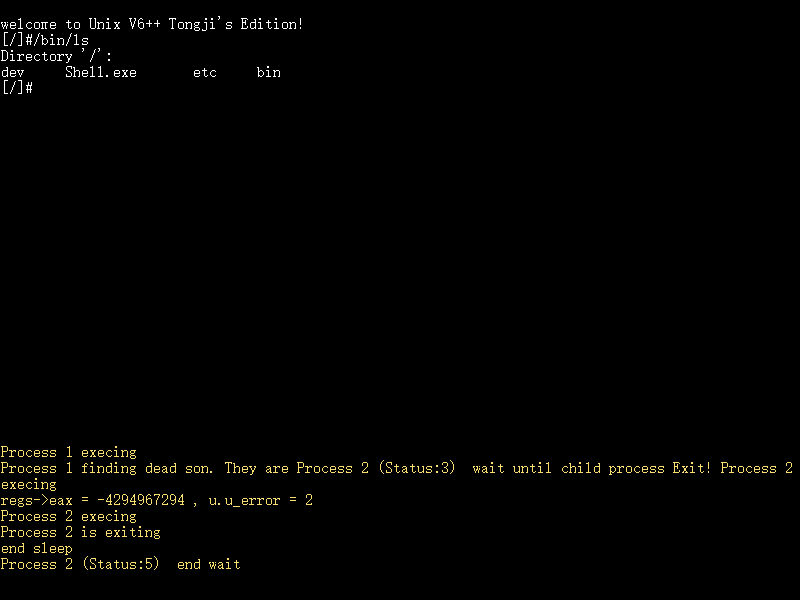
\includegraphics[width=0.85\textwidth]{figures/run_shell.png}
  \caption{系统引导进入 shell 并执行目录列出}
  \label{fig:run-shell}
\end{figure}

\subsection*{用例 2：fork 与进程管理}
执行 \texttt{/bin/fork} 程序，输出 \texttt{My PID is 8}，表明子进程被成功创建；
同时屏幕上可见父进程 \texttt{Process 1} 通过 \texttt{wait} 等待并回收子进程
（\texttt{finding dead son}、\texttt{is exiting}、\texttt{end wait}）的完整日志
（图~\ref{fig:run-fork}）。fork 成功创建子进程、父进程正确回收，证明 fork 的页表
复制、COW 共享页建立、缺页处理与进程生命周期管理在运行时协同工作。

\begin{figure}[H]
  \centering
  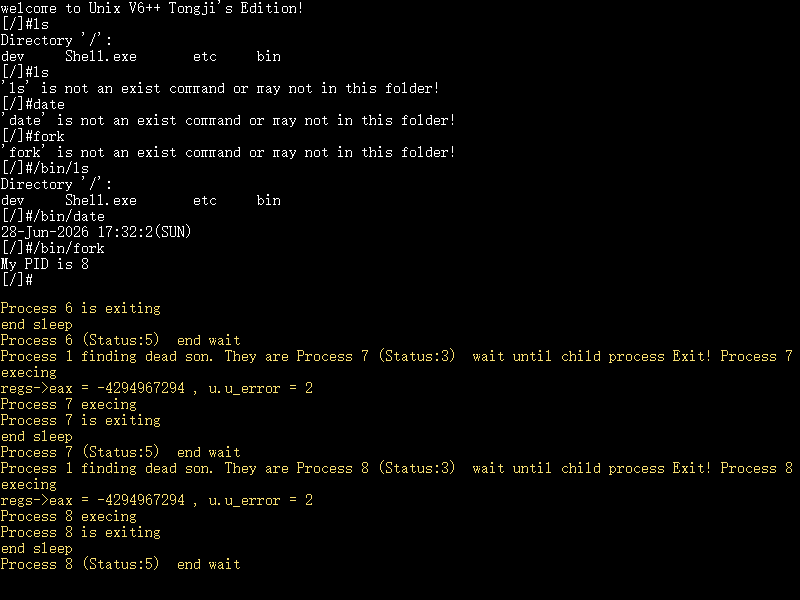
\includegraphics[width=0.85\textwidth]{figures/run_fork.png}
  \caption{执行 /bin/fork：子进程创建与父进程 wait 回收}
  \label{fig:run-fork}
\end{figure}

\subsection*{用例 3：exec 加载用户程序}
执行 \texttt{/bin/date}，程序正确输出当前日期 \texttt{28-Jun-2026}（图~%
\ref{fig:run-exec}）。这表明 \texttt{exec} 能够正确加载用户程序、建立用户页表映射，
并通过参数栈传递命令行参数，验证了第 5.4 节借用 0\# 页表构造参数栈、直接挂用户页表
的机制。

\begin{figure}[H]
  \centering
  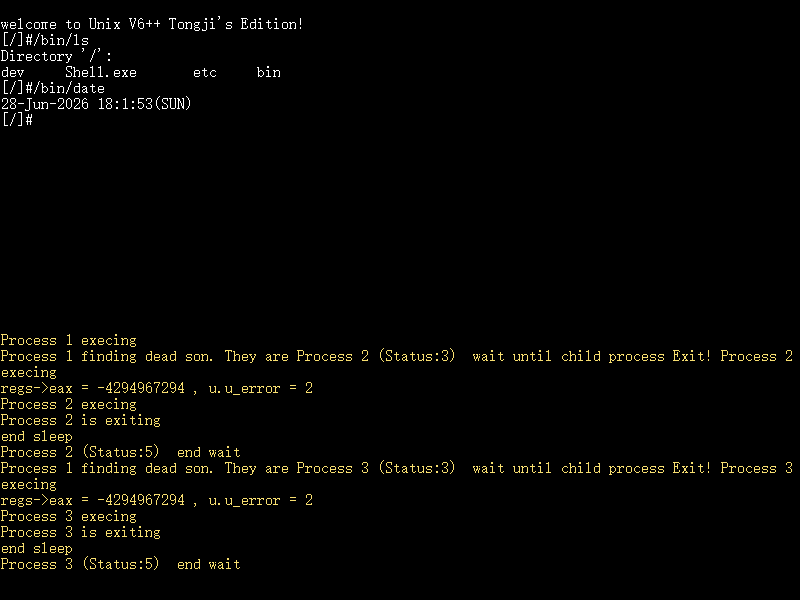
\includegraphics[width=0.85\textwidth]{figures/run_exec.png}
  \caption{执行 /bin/date：exec 加载用户程序并输出}
  \label{fig:run-exec}
\end{figure}

\subsection*{用例 4：正文段共享}
多次执行同一可执行文件时，内核经 \texttt{text} 表复用 \texttt{x\_caddr[]} 记录的
正文段物理页框，不重复分配；进程退出后由 \texttt{x\_ccount} 控制按引用释放。该机制
在上述用例的多次程序加载中均在后台正常工作（系统未出现代码页错误或重复分配导致的
异常），验证了第 5.5 节正文段共享与按计数释放的正确性。

\subsection*{用例 5：位示图分配与回收}
在用例 2、3 中反复执行 \texttt{fork}/\texttt{exec}/\texttt{exit} 的过程中，物理页框
由位示图按需分配、由引用计数 \texttt{Page[]} 控制回收。系统在多次进程创建与退出后
仍稳定运行，未出现页框泄漏或重复分配导致的崩溃，验证了第四章位示图与引用计数协同
的正确性。

\subsection*{验证结果汇总}
表~\ref{tab:test-summary} 汇总各用例的验证点、覆盖机制与实际结果。

\begin{table}[H]
  \centering
  \caption{验证用例与覆盖机制汇总}
  \label{tab:test-summary}
  \begin{tabular}{cllcc}
    \toprule
    序号 & 验证项 & 验证程序 & 覆盖机制 & 结果 \\
    \midrule
    1 & 引导与 shell    & ls             & 页目录/核心页表/位示图初始化 & 通过 \\
    2 & fork / 进程管理 & fork           & COW 建立 + 页表复制 + wait   & 通过 \\
    3 & exec / 参数栈   & date           & 借用 0\# 页表构造参数栈      & 通过 \\
    4 & 正文段共享      & 多次 exec      & text x\_caddr[] + x\_ccount  & 通过 \\
    5 & 页框分配回收    & 反复 fork/exit & 位示图 + Page[] 引用计数     & 通过 \\
    \bottomrule
  \end{tabular}
\end{table}

综上，系统在 QEMU 下成功启动并稳定运行 \texttt{fork}、\texttt{ls}、\texttt{date} 等
用户程序，进程创建、程序加载、页框分配回收等关键路径均表现正常，从运行层面验证了
本次离散化改造未破坏系统功能，且各机制能够协同工作。
         % 第八章  系统测试与验证
% =====================================================================
%  第九章  设计评价与不足
% =====================================================================
\chapter{设计评价与不足}

\section{已完成目标}
本次课程设计围绕 UNIX V6++ 内存管理的离散化展开，已完成课设提出的全部三大改造目标：

\begin{enumerate}
  \item \textbf{页表系统改造}。实现了每进程独立的页目录，进程创建时动态分配页目录并
        写入 \texttt{CR3}；每个进程保留一张私有 1\# 用户页表，核心页表与 0\# 用户页表
        全局共享；进程切换通过 \texttt{SwtchUStruct} 更新内核页表 user 项并刷新
        \texttt{CR3} 完成（第三章）。
  \item \textbf{物理页框分配改为位示图}。以 \texttt{BitMap} 替代连续空闲分区表，
        \texttt{BitMapAllocator} 通过位运算实现离散分配与释放；页表区与用户区分别由
        \texttt{KernelPageManager}/\texttt{UserPageManager} 管理；引入 \texttt{Page[]}
        页引用计数支撑共享页生命周期（第四章）。
  \item \textbf{离散化进程映像管理}。实现了逻辑页离散存放、fork 写时复制、exec 直接
        挂用户页表并构造参数栈、正文段共享（\texttt{Text::x\_caddr[]} 存物理页框号）
        四项要求（第五章）。
\end{enumerate}

在工程层面，本设计同时对构建与运行环境进行了适配，使改造后的内核能够完整构建、
引导启动并运行用户程序，从而具备了在本地验证各机制的条件。

\section{当前实现的优点}
归纳起来，当前实现有如下几个优点。

\textbf{第一，改造层次清晰。}整个设计自然地分为页表层、页框分配层、进程生命周期层
三个相互独立又彼此耦合的层次。页表改造、位示图分配与引用计数各自负责明确的职责：
页表负责虚\,$\to$\,物映射，位示图负责页框的分配回收，引用计数负责描述共享物理页的
生命周期，COW 则把 fork 后的共享页面延迟复制到真正写入时再执行。这种拆分使得系统
可以沿"页表、页框、进程生命周期"三层结构加以解释，而不必把所有逻辑混在某一个函数里。

\textbf{第二，保留了用户态连续地址空间的抽象。}对用户程序而言，text、data、heap 和
stack 仍按熟悉的方式组织，无需感知物理页框是否连续；对内核而言，真实物理内存可以按
4KB 页框离散分配，并由页表重新拼接成连续虚拟空间。这正是分页机制的核心价值，也符合
课设"离散化存储"的目标。

\textbf{第三，fork 采用写时复制。}相比简单复制整个用户映像，COW 既减少了 fork 时的
物理内存复制开销，也能自然地处理父子进程共享页面、后续写入分离、text 段只读共享等
情形；引用计数的加入使页面释放不再只看某一个进程的页表项，而是能判断该物理页是否仍
被其他进程使用。

\textbf{第四，工程可运行性较强。}本设计处理并记录了工具链适配、Makefile 改写、
bootloader 加载、镜像布局等问题，使系统不致停留在代码层面，而是能够启动到 shell 并
运行用户程序。对操作系统课程设计而言，"能构建、能启动、能验证"本身就是实现质量的
重要组成部分。

\section{不足与后续改进}
当前实现仍存在若干不足，在报告中明确说明如下。

\textbf{其一，swap 相关遗留路径未完全清理。}核心用户页框分配、fork/COW、exec/exit 等
运行时主路径已经转向离散页框模型，不再依赖旧的连续进程映像换入换出作为主机制；但原
框架中仍保留 \texttt{SwapperManager} 的若干遗留路径，例如 text 副本、僵尸进程 u 区
保存以及内存不足时的旧接口。这些遗留路径在当前验证范围内并非主路径，但从系统设计
完整性看，后续仍应进一步梳理和清理。

\textbf{其二，ATA 磁盘 I/O 采用同步 PIO 替代 DMA。}这一选择提高了本地 QEMU 验证的
可靠性——因为在离散页表模型下，缓冲区的线性地址不能再通过简单掩码直接得到 DMA 所需
的物理地址；但 PIO 的效率低于 DMA，也没有真正解决"离散页表模型下如何为 DMA 提供正确
物理缓冲区描述"的问题。后续若继续完善，可基于页表查询或专门的 DMA 缓冲区机制，为
ATA DMA 构造可靠的物理地址或 PRD 表。

\textbf{其三，内存不足处理较为粗糙。}bitmap 分配器能够判断页框是否可用，但很多上层
路径仍倾向于假设分配成功，或在失败时直接 panic。一个更完整的系统应当在用户页框不足
时向系统调用返回错误，或实现更明确的进程回收、页面回收、失败回滚策略。由于课设明确
不使用盘交换区，内存不足时如何优雅失败也应成为后续改进重点。

\textbf{其四，自动化测试与文件系统构建工具的跨平台支持不足。}当前的验证以手动用例
为主，缺乏回归测试套件；同时，V6++ 文件系统镜像的构建仍依赖 Windows 专有工具，本地
跨平台生成镜像尚需额外工作。后续可补充自动化测试，并实现基于 \texttt{mtools} 或自研
写入器的跨平台镜像构建方案。
         % 第九章  设计评价与不足
% =====================================================================
%  第十章  总结与体会
% =====================================================================
\chapter{总结与体会}

本次课程设计围绕 UNIX V6++ 的内存管理离散化展开，目标是在教师已有代码基础上，继续
完成页表系统、物理页框分配和进程映像管理的改造，并使系统能够在本地环境中真正运行。
最终实现将原先偏连续映像和相对映射的管理方式，改造成以 4KB 页框为单位的离散页式
管理模型——每进程独立页目录与私有用户页表承担地址映射，位示图承担页框分配，引用
计数与 COW 承担共享页的生命周期与按需复制。

通过本次课程设计，我对操作系统内存管理的理解从"概念层面的分页机制"进一步深入到
"一个可运行内核中各模块如何配合"。页表并不是孤立的数据结构，它会牵动进程切换、
异常处理、exec 参数栈、内核访问用户地址、text 共享释放以及设备 I/O 缓冲区等多条
路径；位示图也不只是一个分配器，它需要和页表项、引用计数以及释放逻辑共同维护物理
页的生命周期。这种"一个数据结构的改变会沿控制流扩散到许多看似无关的地方"的体验，
是单纯阅读教材难以获得的。

调试过程也让我认识到，内核问题往往不能只看故障发生的最后一行。一次 kernel page
fault 可能真正来自 fork 时引用计数漏加，也可能来自 text 释放范围错误，还可能来自
信号返回时恢复了错误的栈帧；一次用户程序参数丢失，也不一定是 shell 解析错误，而可能
是 exec 构造新栈时写入了错误的页表映射。只有沿着完整的执行路径分析，才能把现象和
根因正确对应起来。报告第七章列出的几个问题，正是这一认识的具象化。

此外，本次项目让我体会到工程环境对操作系统实验的重要性。中文路径、陈旧构建缓存、
Makefile 命令差异、bootloader 加载扇区数不足、磁盘镜像布局不一致，都可能造成看似
"内核崩溃"的现象。对于底层系统项目而言，稳定的构建和运行环境本身就是调试能力的一部
分——先排除工程层面的干扰，才能让真正的算法缺陷显露出来。

总体而言，本次课程设计完成了 UNIX V6++ 内存管理从连续映像思路到离散页框管理思路的
核心转变。虽然当前实现仍保留了部分历史路径，在内存不足处理、DMA 支持和自动化测试等
方面还有后续改进空间，但系统已经具备在本地构建、启动并展示页表、位示图、COW 与离散化
进程映像管理等主要机制的条件。通过这次实现与调试，我对操作系统内核中"抽象设计"与
"工程落地"之间的关系有了更具体的理解。

\clearpage
   % 第十章  总结与体会

% ---------- 参考文献 ----------
\backmatter
% =====================================================================
%  参考文献 —— 用 enumerate 手动排版, 避免该bibliography 的跳页问题
% =====================================================================
\clearpage
\phantomsection
\addcontentsline{toc}{chapter}{参考文献}
\begin{center}
{\huge\bfseries 参考文献}\par
\end{center}
\vspace{1.2em}

\begin{enumerate}[label={[\arabic*]},leftmargin=2.6em,itemsep=4pt]

  \item Lions J. \emph{Commentary on UNIX 6th Edition Source Code}[M].
        上海: 同济大学计算机系讲义.

  \item 方钰. \emph{UNIX V6++ 内核源代码与课程设计讲义}[Z].
        同济大学计算机科学与技术学院, 2026.

  \item Intel Corporation. \emph{Intel 64 and IA-32 Architectures Software
        Developer's Manual, Volume 3: System Programming Guide}[Z].

  \item 李治军, 刘宏伟. \emph{操作系统原理、实现与实践}[M].
        北京: 高等教育出版社.

  \item The Bochs Project. \emph{Bochs IA-32 Emulator Project}[EB/OL].
        \url{http://bochs.sourceforge.net/}.

  \item Bellard F. \emph{QEMU, a Fast and Portable Dynamic Translator}[EB/OL].
        \url{https://www.qemu.org/}.

\end{enumerate}


\end{document}
